\documentclass[11pt,a4paper]{article}
\usepackage[T1]{fontenc}
\usepackage[utf8]{inputenc}
\usepackage{lmodern}
\usepackage[margin=2.5cm]{geometry}
\usepackage{booktabs,longtable,array,graphicx,url,setspace,caption,enumitem,float,pdflscape}
\usepackage[hidelinks]{hyperref}
\setstretch{1.15}
\captionsetup{font=small,labelfont=bf}
\newcommand{\todo}[1]{\textbf{[#1]}}
\makeatletter\g@addto@macro\UrlBreaks{\do\.\do\-\do\_\do\(\do\)\do\;}\makeatother
\setlength{\parskip}{0.3em}

\title{Do the gains from digital technology waves differ by income level?\\ A pilot evidence map of cross-country studies}
\author{}
\date{}

\begin{document}
\maketitle


\begin{abstract}
\noindent\textbf{Background.} Mobile telephony, the internet and, more recently, artificial intelligence (AI) are often expected to widen or narrow income gaps between countries, but the empirical cross-country evidence has not been mapped across outcomes. \textbf{Methods.} We built a pilot evidence map of empirical cross-country studies that relate ICT, mobile, internet, broadband and AI to output, structural change, labour markets, distribution, living standards and resource use. Records came from OpenAlex, Crossref, NBER and the first page of four Google Scholar queries; Scopus, Web of Science and EconLit were not searched, so the search is incomplete. One reviewer assisted by language models screened records and extracted study characteristics and results, which were cross-checked by a second model run and, for the estimates behind the one pooled figure, by the author against the source papers. Risk of bias was rated with an adapted ROBINS-I tool, and the evidence is described by outcome family, technology stream, income coverage and design. \textbf{Results.} Of 132 full texts assessed, 88 studies were included (71 on ICT, mobile, internet and broadband; 15 on AI; 2 on both). None was at low risk of bias (moderate 10, serious 67, critical 11). Fifty-three studies report output or productivity outcomes, and most report a positive association, but the sign is not uniform. A descriptive pooled partial correlation from 22 studies is 0.16 (95\% CI 0.09 to 0.23, I$^2$ 93\%); it depends on the studies found, falls to 0.04--0.09 after adjustment for small-study bias, and moderator analyses were unstable and are not interpreted. Thirty-eight studies compare income groups or regions: nine find larger effects in richer economies, eleven in poorer ones, and four find no difference, mostly without a formal test. Authors most often test human capital, finance, governance and infrastructure as conditions. Only two of 17 AI studies include a low-income economy. A supplementary check with World Bank mobile data gives answers that depend on the specification. \textbf{Conclusions.} The evidence cannot show whether rich or poor economies gain more. The contribution is a map of where evidence exists and how credible it is; the main gaps are credible identification for low- and middle-income economies and realised-use measures for AI.
\par\medskip\noindent\textbf{Keywords:} digital technology; artificial intelligence; income level; evidence map; productivity.\\
\textbf{JEL codes:} O33, O47, O11, L96.
\end{abstract}

\newpage

\section{Introduction}

Whether new technologies narrow or widen income gaps between countries is a long-standing question, and it has returned with artificial intelligence. Early empirical work found sizeable output effects of telecommunications infrastructure \cite{roller2001}. Later work on the long-run diffusion of technologies finds that technologies arrive at similar times in rich and poor countries, but that the intensity of their use diverges \cite{comin2010,comin2018}. If so, the gains from a new technology should depend on a country's conditions at the time of adoption, and not only on whether the technology has arrived.

Evidence on this is scattered. Studies use different technologies (mobile subscriptions, internet users, composite ICT indices, ICT capital, robots, AI readiness indices), different outcomes (growth, productivity, employment, inequality, human development, emissions), different samples and different estimators. Individual studies often report one average effect and one or two interaction terms. A reader who wants to know whether a low-income economy can expect the same payoff as a high-income one has no single place to look, and a policymaker who reads one study can reach the opposite conclusion from one who reads another.

We therefore ask: \emph{in empirical cross-country studies of digital and general-purpose technology waves, what do we know about the effects on output, structural change, labour markets, distribution, living standards and resource use, do the effects differ by income level and by country characteristics, and how credible is the evidence?} We keep studies of historical waves (ICT, mobile, internet, broadband, crypto-assets) separate from studies of AI, because AI evidence is younger and thinner.

This paper is a pilot evidence map. It is not a complete systematic review: the search covered three databases and a small part of Google Scholar, and a single reviewer assisted by language models screened and extracted the studies. The map describes the included studies by outcome family, technology stream, income coverage and design, rates the risk of bias of each study, and reports one descriptive pooled association for the best-covered question, the association between ICT-type adoption and output. A short supplementary analysis of World Bank mobile-phone data shows how a simple version of the question behaves under different specifications.

The contribution is a transparent map of where cross-country evidence exists and where it does not, with a quality rating of each study and a count of the income-group comparisons. We are explicit about what the evidence cannot show. Data and code availability is described in the Declarations.

The rest of the paper is organised as follows. Section~\ref{sec:background} sets out the conceptual background and the questions. Section~\ref{sec:methods} describes the methods. Section~\ref{sec:results} reports the map, Section~\ref{sec:panel} the supplementary panel check, and Section~\ref{sec:discussion} discusses the findings. Sections~\ref{sec:limits} and~\ref{sec:conclusion} give the limitations and conclusions.

\section{Conceptual background and questions}\label{sec:background}

\subsection{Why the same technology could pay differently}
Four mechanisms recur in the literature on information and communication technology and on automation, and each implies a reason why the gain from a technology might differ by income level.

\emph{Infrastructure and complementary investment.} Telecommunications infrastructure raises output, and the effect may depend on how much infrastructure already exists, because network benefits grow with the size of the network \cite{roller2001}. Where electricity, roads and financial services are scarce, the same handset or connection may yield less. This implies that the gain depends on a country's stock of complementary assets, which is usually lower in poorer economies.

\emph{Information and market access.} Mobile phones can reduce price dispersion and waste where markets are thin. In a study of South Indian fisheries, the arrival of mobile phones reduced price dispersion and waste and raised welfare \cite{jensen2007}, and a review of evidence from Africa describes how mobile phones can improve information flows in agricultural and other markets \cite{aker2010}. These mechanisms are strongest where information was previously scarce, which is more common in lower-income settings, and they imply large early gains at low adoption levels.

\emph{Skills and tasks.} Computers substitute for routine tasks and complement non-routine tasks \cite{autor2003}, and automation both displaces and creates tasks \cite{acemoglu2019}. In Africa, the arrival of fast internet through submarine cables was associated with higher employment, and the effect was larger for more skilled workers \cite{hjort2019}. The gains therefore depend on the skills of the workforce, which differ by income level.

\emph{Absorptive capacity.} The ability to use external knowledge depends on prior related knowledge \cite{cohen1990}. For technology adoption this means that returns depend on human capital, management capacity and institutions, again variables that differ systematically by income.

Two forces therefore pull in different directions. Catch-up and early information gains suggest that low-adoption, lower-income economies could gain more per unit of adoption. Complementary assets, skills and absorptive capacity suggest that higher-income economies could gain more. A third consideration is time: the long-run diffusion evidence suggests that gains may build over years, and a short window may miss them \cite{comin2018}. A review of the empirical evidence on information technology and economic performance, published early in the period we study, describes the findings as mixed \cite{dedrick2003}; it is not an estimating study and is not among our included studies.


\subsection{Questions}
These mechanisms lead to four questions that structure the map. We do not test hypotheses: the design cannot support causal or confirmatory inference, and the mechanisms predict effects of opposite sign.

\begin{description}[leftmargin=1.6em,itemsep=2pt]
\item[Q1] Is ICT-type adoption associated with higher output and productivity in cross-country studies, and how large and how consistent is the association?
\item[Q2] Do studies find that the association differs by income level, and in which direction?
\item[Q3] Which enabling conditions (human capital, financial depth, governance, infrastructure) do authors test, and do they find that the condition raises or lowers the association?
\item[Q4] How credible is the evidence (design and risk of bias), how does the AI evidence compare with the evidence on earlier technologies, and where are the gaps by outcome and income group?
\end{description}

\section{Methods}\label{sec:methods}

\subsection{Protocol and registration}
The study was planned as a systematic review following PRISMA 2020 \cite{prisma2020} and the structure of PRISMA-P \cite{prismap}, with a written protocol (version 1.0, 2 October 2026) available through the data and code link in the Declarations. The protocol was not registered before the search, the search turned out to be incomplete (see below), and one reviewer screened the records. We therefore report the study as a pilot evidence map and use PRISMA 2020 items as a reporting guide, not as a claim of compliance. Amendments made after the search are listed in Appendix~\ref{app:amend}.

\subsection{Eligibility criteria}
We included quantitative empirical studies with their own estimation (panel regression, instrumental variables, growth accounting, event studies, structural estimation) that relate adoption, diffusion, investment or capability of ICT in general, mobile telephony, internet or broadband, crypto-assets or AI to at least one outcome in six families: (1) output and productivity, (2) structural change, (3) labour market, (4) poverty and distribution, (5) living standards beyond income (consumption, health, schooling, financial inclusion) and (6) resource cost (electricity use, carbon intensity). Historical-wave studies needed at least 10 economies or an explicit income-group comparison; AI studies needed at least 3 economies or an income-level comparison. Studies from 1995 onward in English were eligible. Purely conceptual papers, reviews and studies whose only outcome was adoption itself were not synthesised. Full criteria and exclusion codes are in Appendix~\ref{app:criteria}.
We included quantitative empirical studies with their own estimation (panel regression, instrumental variables, growth accounting, event studies, structural estimation) that relate adoption, diffusion, investment or capability of ICT in general, mobile telephony, internet or broadband, crypto-assets or AI to at least one outcome in six families: (1) output and productivity, (2) structural change, (3) labour market, (4) poverty and distribution, (5) living standards beyond income (consumption, health, schooling, financial inclusion) and (6) resource cost (electricity use, carbon intensity). Historical-wave studies needed at least 10 economies or an explicit income-group comparison; AI studies needed at least 3 economies or an income-level comparison. Studies from 1995 onward in English were eligible. Purely conceptual papers, reviews and studies whose only outcome was adoption itself were not synthesised. Full criteria and exclusion codes are in Appendix~\ref{app:criteria}.
\subsection{Information sources and search}
We searched OpenAlex (a Boolean query restricted to the economics field), Crossref (96 technology-by-context queries) and the NBER working-paper series, covering 1995 to the search date of 2 October 2026. The search blocks and the OpenAlex query are in Appendix~\ref{app:search}. arXiv was attempted but did not respond in usable time. Scopus, Web of Science and EconLit were not searched, because they need institutional access. After removing duplicates by DOI and by normalised title and year, 3,612 records remained.

A blind re-screening of the retrieved records suggested that the search had missed relevant studies (Section~\ref{sec:crosscheck}). A supplementary check in Google Scholar, where the author ran four of 15 planned queries (G1, G2, G4 and G7, listed in Appendix~\ref{app:search}) and passed on the first page of 10 results for each, found that most results were not among the 3,612 records (9 of 10 for G1, 6 of 10 for G2, 7 of 10 for G4 and 7 of 10 for G7); of two further results that were among them, one (Yin and Choi 2023) had been removed by the automated stage-1 rule and the other (Gonzales 2023) had been judged includable but never read for lack of a full text. These records are handled outside the main flow (Table~\ref{tab:prisma}). Eleven planned queries have not been run, and the search as a whole should therefore be regarded as incomplete.


\subsection{Screening and full-text access}
One reviewer, assisted by language models, screened the records. Automated rules removed records with no eligible technology term, no outcome term or no multi-economy cue (stage 1). Title and abstract screening then applied the eligibility criteria, with four holding categories for records that were not eligible but useful (context on diffusion, environmental-only outcomes, reviews for citation search and supplementary micro evidence). No second human screener was available. Instead, a separate model run, which saw only the criteria and each record's title and abstract, independently re-screened a random sample of 340 records (100 of those removed by the automated rules, 120 of those removed at title level and 120 of those assessed at abstract level). Records the first screener excluded and the second would include were adjudicated by a third blind reading of the abstract. Agreement and an estimate of missed records are reported in the Results.

Full texts were obtained from open-access sources, repositories and the author. Records without a free full text, and those the author judged to come from unreliable venues, were not read and are not used as evidence. This favours open-access studies; Section~\ref{sec:limits} discusses it. Studies supplied by the author after the search, records flagged by the re-screening and records from the Google Scholar pages were read and handled in the same way as the others. Of the twenty studies from the Google Scholar pages that could be downloaded, three were excluded at full text (a five-country panel, a mathematical model without estimation, and a study estimated only on a simulated panel), and one was kept on the strength of its generic ICT index alone, because it does not measure AI. Three further results of the first query could not be obtained.

\subsection{Data extraction and verification}
For each included study we extracted technology, exposure measure, sample, estimator, identification strategy, results by outcome family with printed estimates and uncertainty, heterogeneity findings and group-specific results, using a fixed form (Appendix~\ref{app:criteria}). A language model read the converted full text of each study and recorded each item with a page or table locator and a short quote. The extraction was cross-checked in four ways. First, an automatic check compared quotes with the text (515 of 756 quotes matched verbatim; the rest were affected by table layout and paraphrase). Second, a separate model run re-read each of the 88 included records and each of the 317 extracted regression estimates against the full text and classified every item as confirmed, corrected or unverifiable. This catches transcription and reading errors, but the same family of model reads the same converted text, so it is not an independent check. Third, a separate model run re-extracted key fields blind for 16 randomly chosen studies and we compared the two extractions. Fourth, the author checked samples of the extracted data by hand against the source papers and verified each of the 22 estimates behind the pooled figure reported below. \todo{author: after the check, state the number of studies verified and the number of corrections}

\subsection{Risk of bias}
Risk of bias used a six-domain tool adapted from ROBINS-I \cite{robinsi}: confounding and reverse causation, exposure measurement, selection of countries and years, outcome measurement, specification and researcher degrees of freedom, and selective reporting. The overall rating was low, moderate, serious or critical, with the definitions in Appendix~\ref{app:criteria}. One rater made the ratings; the cross-check offered an opinion on each, which we report without changing the ratings.

\subsection{Synthesis}
We describe the studies by outcome family, technology stream, income coverage and design, following the SWiM reporting guideline \cite{swim}. Studies were grouped by outcome family, and within each family we tabulated the direction of the results, the estimator, the sample and the risk of bias (Appendix~\ref{app:families}). Counts of study directions are descriptive; they are not weighted by sample size or quality and are not effect sizes. For output and productivity, we also computed one descriptive pooled association. Each headline estimate of ICT-type adoption on output or productivity was converted to a partial correlation coefficient, $PCC = t/\sqrt{t^2 + df}$ \cite{stanley2012}, with $df$ equal to the number of observations minus 10, and one headline estimate per study was pooled by random effects \cite{dersimonian1986}. Estimates reported only with $p$-values or intervals, interaction terms and non-ICT exposures were not converted. The pooled value is a summary of the studies we found, not an estimate of a population effect, and its sensitivity to the studies included is reported in Appendix~\ref{app:sens}. Moderator regressions and publication-bias tests \cite{stanley2014} were run as sensitivity analyses; they were unstable and are not interpreted (Appendix~\ref{app:sens}).

\subsection{Supplementary macro-panel check}
To see how a simple version of the income question behaves under different specifications, we used public World Bank World Development Indicators for 1995 to 2019 and mobile subscriptions per 100 people as the technology measure. The specifications were fixed-effects panels in five-year periods (same-period and predetermined change in adoption, by current income group), a staggered event study around the year mobile subscriptions reach 10 per 100 people with not-yet-treated controls \cite{callaway2021,sun2021,dechaisemartin2020}, and local projections \cite{jorda2005}. All of these are associations. We have no instrument and make no causal claim. The design, variables and full results are in Appendix~\ref{app:panel}.


\section{Results of the evidence map}\label{sec:results}

\subsection{Study selection}
Figure~\ref{fig:prisma} and Table~\ref{tab:prisma} give the flow. Of 247 records sent to full-text assessment, 106 full texts were obtained and read, together with one review, five records outside the 247 that the blind re-screening flagged (Section~\ref{sec:crosscheck}) and twenty records found through Google Scholar. After the cross-check, 88 studies are included, 43 were excluded at full text (14 for too few economies, 5 for an ineligible exposure, 1 for an ineligible outcome, 23 for being conceptual or lacking their own estimation) and one was kept as context. Four studies were moved from include to exclude after the cross-check, on eligibility grounds (no own estimation, an undetermined number of economies, outcomes outside the six families, too few economies). About 140 of the 247 records have not been read because no free full text was available.

\begin{figure}[ht]\centering
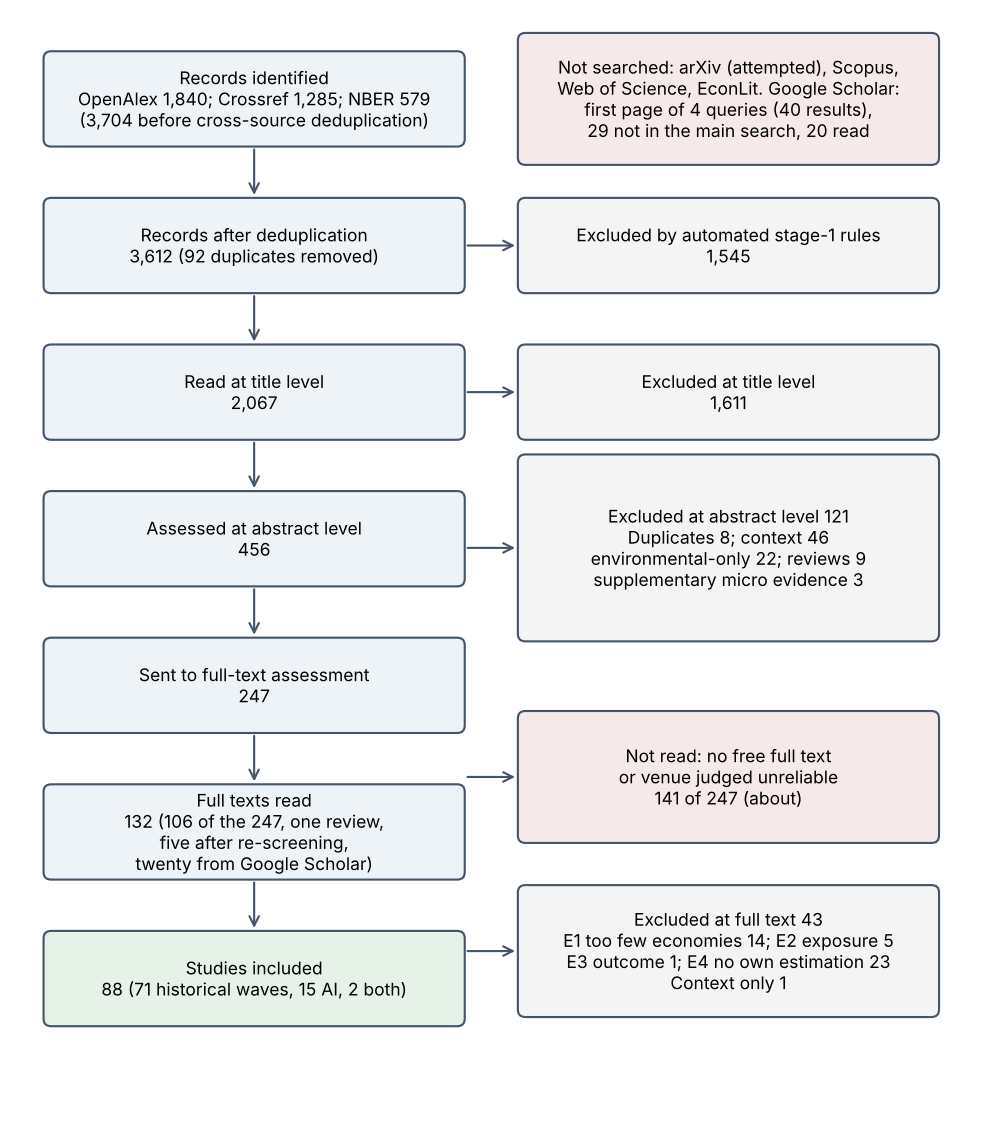
\includegraphics[width=0.78\textwidth]{fig_prisma.png}
\caption{PRISMA 2020 flow diagram.}\label{fig:prisma}
\end{figure}

\begin{table}[ht]\centering\small
\caption{Study selection (counts as recorded by the author).}\label{tab:prisma}
\begin{tabular}{@{}p{12.2cm}r@{}}\toprule
Stage & n\\\midrule
Records identified (OpenAlex 1,840; Crossref 1,285; NBER 579; before cross-source deduplication 3,704) & 3,704\\
Duplicates removed across sources & 92\\
Records after deduplication & 3,612\\
Google Scholar, queries G1, G2, G4 and G7, first page each (supplementary): results / not in the main search / obtained and read & 40 / 29 / 20\\
Excluded by automated stage-1 rules & 1,545\\
Read at title level / excluded at title level & 2,067 / 1,611\\
Assessed at abstract level / excluded at abstract level & 456 / 121\\
Held as duplicates, context, environmental-only, reviews, supplementary & 88\\
Sent to full-text assessment & 247\\
Full texts read (106 of the 247, one review, five records added after the re-screening and twenty from Google Scholar) & 132\\
Excluded at full text & 43\\
Kept as context only & 1\\
\textbf{Included} & \textbf{88}\\\bottomrule
\end{tabular}\end{table}

\subsection{Characteristics of included studies}
The 88 included studies were published between 2003 and 2026, and 70 of them from 2020 onward (Figure~\ref{fig:years}). Seventy-one study ICT, mobile, internet or broadband; 15 study AI; 2 cover both. Most use country-year panels (70), with a few at industry-country level. In a rough classification of the main estimator, 35 use system or difference GMM, 32 use fixed-effects, random-effects or pooled OLS, 13 use ARDL, cointegration or heterogeneous-panel estimators and 8 use growth accounting, data envelopment or other methods. Forty-two studies have no identification strategy beyond controls and fixed effects. Twenty-eight list at least one low-income economy; studies that do not state their income coverage are counted as not listing one. Outcome families, with a study able to contribute to several, are: output and productivity 53, labour market 15, living standards beyond income 16, poverty and distribution 13, structural change 6, resource cost 6. Appendix~\ref{app:studies} lists all studies and Appendix~\ref{app:families} gives the results by family.

\begin{figure}[ht]\centering
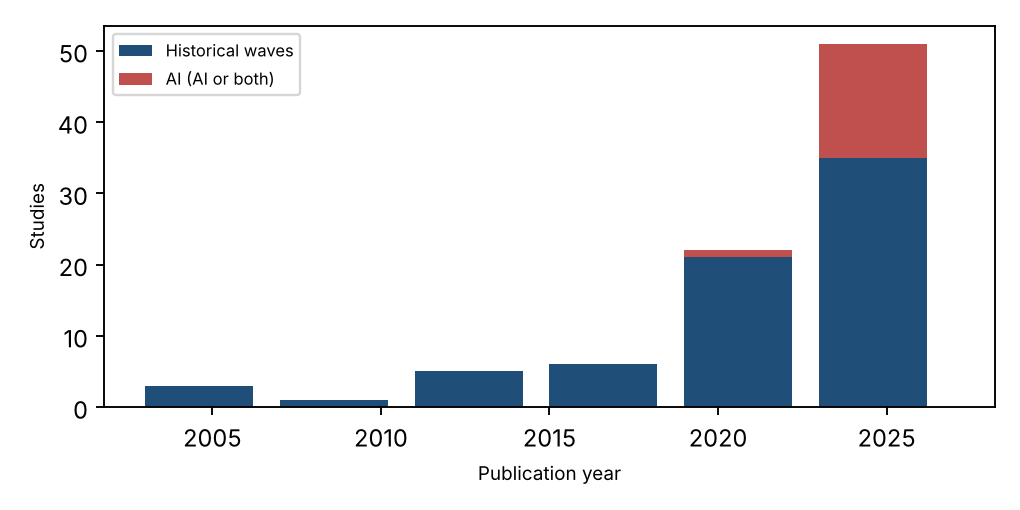
\includegraphics[width=0.62\textwidth]{fig_years.png}
\caption{Included studies by publication year and stream.}\label{fig:years}
\end{figure}

\subsection{Risk of bias}
No study was rated at low risk of bias. The ratings were moderate for 10 studies, serious for 67 and critical for 11 (Figure~\ref{fig:rob}). In the cross-check, the separate reader disagreed with the overall rating for 11 of 88 studies (seven too harsh, four too lenient); we did not change any rating. The commonest weaknesses are adoption treated as exogenous, indices whose scope does not match the technology, and many specifications with no stated preferred one.

\begin{figure}[ht]\centering
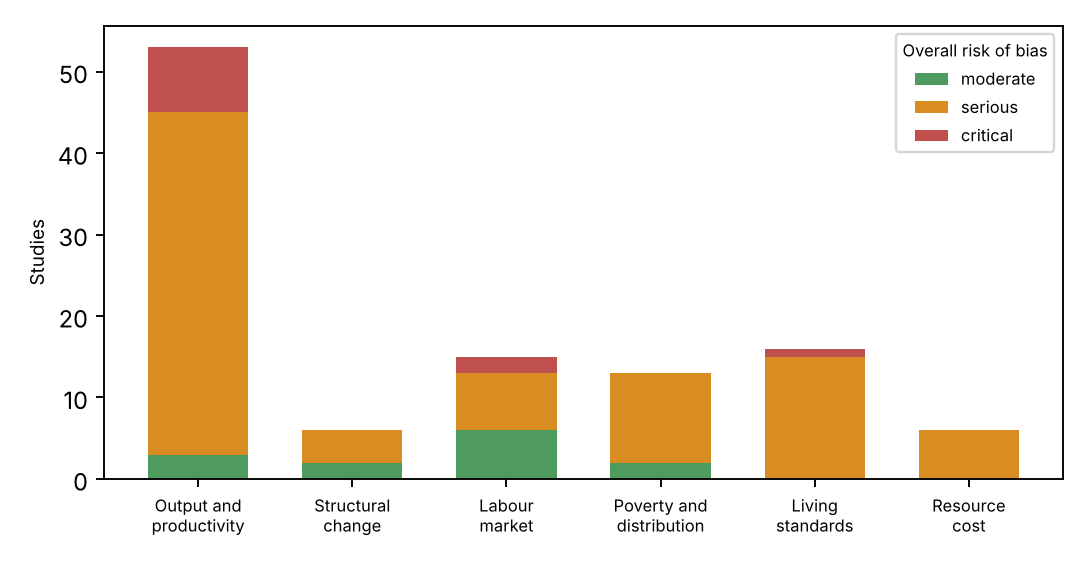
\includegraphics[width=0.66\textwidth]{fig_rob.png}
\caption{Overall risk of bias by outcome family (a study counts in each family it reports).}\label{fig:rob}
\end{figure}


\subsection{Verification of screening and extraction}\label{sec:crosscheck}
In the cross-check by a separate model run, 492 of 531 result entries in the 88 included records were confirmed, 34 were corrected and 5 could not be verified; 18 of 170 heterogeneity entries were corrected. Of 317 regression estimates, 311 matched the printed tables and six needed correction: one income label, and five estimates of Saba and Ngepah (2022), which had been read from the wrong cell of a panel-VAR table (rows are equations and columns are lagged regressors, as the paper's own causality tests show, whereas its text reads the table the other way). The extraction had followed the paper's text, so the cross-check caught an error that originated in the source. Corrections were applied to the data. Because both passes used the same family of model reading the same converted text, the author's checks against the source papers are the reference.

\emph{Screening.} The blind second screener agreed with the first on whether to send a record to full text for 79\% of the 120 records in the abstract-stage sample (Cohen's kappa 0.59 when its ``unsure'' counts as include and 0.54 when it does not). Its disagreements were mostly cases where it was more inclusive: of the 72 records the first screener did not send forward, it would have included or flagged 20. Of the 8 sampled records the first screener set aside as environmental-outcome-only (protocol amendment 2), the second screener would have sent 7 to full text. Carbon and electricity outcomes are in outcome family 6, so such records meet the eligibility criteria; setting them aside was a prioritisation choice, and it explains in part why only four included studies report resource-cost outcomes.

\emph{Recall.} Among the records excluded earlier, the second screener would have included or flagged 7 of 100 (automated rules), 15 of 120 (title level) and 8 of 120 (abstract level, coded exclusions). After a third blind reading of the abstracts, 2 of 100, 10 of 120 and 4 of 120 met or probably met the criteria. Extrapolated, this implies roughly 31 (range 9 to 108), 134 (74 to 236) and 15 (6 to 38) missed records at the three stages, on the order of 180 in total (range about 90 to 380). These are small samples read by model readers, and 9 of the 30 adjudicated records had no abstract, so the figure is a warning about recall and not a count. Later first-page checks of four Google Scholar queries found 29 of 40 results missing from the 3,612 records (and two more removed by the stage-1 rule or never read), and seventeen of the twenty studies read from them were included, so the main search had poor recall for this question and the estimate above is a lower bound. The missed records are typically AI or digital-economy panels with carbon or energy outcomes, small AI panels, and financial-inclusion studies in Africa and the Arab world. Adding some such studies changed the pooled and moderator results (Appendix~\ref{app:sens}), so conclusions that rest on them are fragile, and the evidence base is smaller than the literature.

\emph{Extraction.} A blind re-extraction of key fields for 16 random included studies agreed with the original on the outcome families (16 of 16), start and end year (15 of 16 each), the presence of an identification strategy (14 of 16), the direction of the headline output result (14 of 16), the number of economies within 5\% (13 of 16), whether the estimator is GMM (13 of 16), the four-way estimator class (12 of 16), whether income groups are compared (12 of 16), and the overall risk-of-bias rating (11 of 16). Low-income coverage agreed in all 5 studies where the blind reader could judge it. Disagreements arise from papers with several estimators, differing sample counts in the text and the tables, and the subjective risk-of-bias scale: where the two differ on risk of bias, the blind reader is more lenient in four of five cases, in line with the cross-check opinions. We therefore treat the estimator classes and risk-of-bias ratings as approximate, and the count of studies that list a low-income economy (28) as uncertain by a few studies.

\subsection{Output and productivity}
Fifty-three studies cover output or productivity (7 on AI). Most report a positive association, but the sign is not uniform: current and lagged mobile effects have opposite signs in one 41-economy GMM study (Chatterjee, 2020); ten high-income countries show no significant effect of any ICT indicator (Satrianto and Ikhsan, 2023); and in 27 EU states the digitalisation coefficient loses significance once economic freedom is added (Balashova, 2023). In 11 MENA economies, CS-ARDL estimates of an ICT index on GDP per capita are 0.05 (long run) and 0.06 (short run), both significant only at 10\%, while the dynamic common correlated effects estimate is 0.30; the paper's own causality tests show feedback in both directions (Dahmani et al., 2023). A digital economy index lowers green total factor productivity across 40 Belt and Road economies (Wang and Ren, 2023), although that outcome sits closer to resource cost.

The studies found later through Google Scholar are no more uniform. Internet use is negatively associated with growth of GDP per capita across 78 economies, significantly so only in the high-income group ($-0.021$, against $-0.012$ pooled and $+0.006$, not significant, in lower-middle income economies; Samariya et al., 2026). An instrumental-variable study of 123 economies finds positive elasticities of GDP per capita with respect to an ICT index in all three income groups, largest in middle-income economies (0.42), then low-income (0.16) and high-income (0.09) (Appiah-Otoo and Song, 2021). A study of the ten ASEAN economies, none of them low-income, finds fixed broadband positively and mobile broadband negatively associated with GDP per capita (Abdelhak et al., 2026). A study of 85 low- and high-income economies finds small positive associations of internet users and fixed telephones with GDP per capita in both groups and a negative association of secure internet servers in low-income economies (Kumari and Singh, 2024). In 182 regions of 27 EU countries, internet use and e-government are mostly positively associated with total factor productivity, with some negative interactions (Rehman and Nunziante, 2023). A study of 45 developed and developing countries finds that the output elasticity of IT is similar across the two groups, with a larger complementarity with tertiary education in developing countries (Dedrick et al., 2013). A study of 42 sub-Saharan economies reports that an ICT index, a technology-readiness index and the share of technology imports are positively associated with growth of GDP per capita, although the paper never measures AI, its stated subject, and is rated critical (Maswana, 2024); a composite digital index is positively associated with output per worker and with GNI per capita in 25 economies (Aly, 2022). Studies of sub-Saharan Africa (Asongu and Acha-Anyi, 2020) and of transition economies (Huang et al., 2008) find thresholds, an inverted U above about 100 mobile subscriptions per 100 people in the first and a level-dependent interaction between IT investment and staff in the second, the latter rated critical. A subnational study of about 34,000 districts in 120 countries finds that expansion of mobile coverage raises nightlight growth, a proxy for local activity, which the author converts to an implied GDP elasticity of 0.018 to 0.023 using an external nightlights-GDP elasticity; the 2G effect is concentrated in developing countries and effects are larger where fixed-line telephone penetration was low (Mensah, 2023). Two panel-VAR studies (9103 and 9104) report only $p$-values, so they could not enter the pooled estimate, and in both the text disagrees with the table. In Saba et al. (2024) the abstract reports a positive effect of ICT on growth, but the printed table shows negative coefficients of lagged ICT on real GDP in the full sample, sub-Saharan Africa and Latin America and a positive one only in the Middle East and North Africa; read with the layout the paper's own Granger tests imply, Saba and Ngepah (2022) shows positive effects of lagged ICT on real GDP in all four income groups, although the outcome is a level in billions of dollars and the coefficients are not comparable across groups.

Interaction terms are the most repeated finding: ICT pays more where human capital is higher in two Asian GMM studies (Mehmood and Azim (2013) and Mehmood and Azim (2014), which share authors, panel and index), a developing-country productivity study, and in Africa, where the effect of the digital economy is negative below a human-capital index of about 2.35 and the average country is below it. Financial development, trade openness, governance, electricity and the diffusion level of ICT also appear as moderators. These are conditional associations from single-equation panels and do not show that raising a moderator would change the return. A non-parametric study of 24 OECD economies finds that ICT capital change has no contemporaneous effect on the production frontier and a positive effect five years later, which supports the view that timing matters. In the five AI studies, developed economies show about twice the productivity effect of emerging economies (0.24 against 0.11) in a 10-economy comparison rated at critical risk of bias; in 63 low and lower-middle income economies, AI-related imports are associated with higher labour productivity, more so where connectivity, electricity and financial inclusion are better; and two further studies (a sub-Saharan firm-level study and a three-country generative-AI survey) are rated critical and cannot be relied on. A study of nine economies (the G7, China and Korea) finds mostly null or sign-changing associations between an AI proxy and GDP per capita, and the proxy in some models is an ICT export share (Özocaklı, 2026).

\subsection{Structural change}
Six studies cover structural change. Internet penetration is associated with faster structural change in a 51-economy panel, more so in low and lower-middle income and agrarian economies than in upper-middle and high-income ones, and more so where forward value-chain linkages are higher; manufacturing employment falls in South Asia and is unchanged in sub-Saharan Africa. A 3G coverage study in 14 developing countries finds jobs created in services and non-farm self-employment but no shift of labour away from agriculture. ICT is positive for industry and services value added but not for agriculture in a 26-economy PMG study, although columns 2 to 4 of its Tables 10 and 11 are identical across industry and services, which casts doubt on the table. A study of about 100 developing economies finds that ICT lowers export concentration, with a larger effect in the low and lower-middle income group ($-0.155$ on the concentration index) than in the high and upper-middle group ($-0.020$), but no formal test of the difference. A panel VAR of 171 economies (Saba and Ngepah, 2022) finds, on a reading consistent with its table layout, a weakly positive association of lagged ICT with the manufacturing share in every income group, whereas its authors read the table as a large negative effect of ICT on industrialisation. The evidence base here is still small.

\subsection{Labour market}
Fourteen studies cover labour markets, five of them on AI. In advanced economies ICT is linked to routine-task decline and polarisation, and capital-skill complementarity raises skill premia. In 27 European countries ICT capital creates more jobs where the share of high-skilled jobs is lower. No included study measures routinisation in low-income economies. Third-generation mobile coverage raises women's labour-force participation but not men's in 14 low- and middle-income countries, in one of the few studies that uses an instrument for developing-country labour outcomes. AI exposure is positively associated with employment growth, concentrated in high-education occupations and younger workers, in European samples; in Southeast Asia the pattern differs by country, though the country-level estimates are shown only in a figure. Across 29 countries, the AI index effect on employment declines with labour productivity level. A 78-economy readiness-index study is rated critical. The pattern across studies is that AI complements skills and displaces the rest, and the evidence on low-income economies is nil.

\subsection{Poverty and distribution}
Twelve studies cover poverty and distribution, two on AI. Results split. In 19 G20 economies, internet use is associated with a lower Gini coefficient in the middle-income group ($-0.020$) and a higher one in the high-income group ($+0.047$), with split samples and no formal test of the difference (Yin and Choi, 2023). A threshold model for 45 developing countries finds that ICT raises the Gini coefficient below a digital-maturity score of 0.48 and lowers it above, an inverted U. In 48 sub-Saharan African economies ICT is positively associated with a composite inclusive-growth index (0.03 to 0.15 across specifications), with trade openness negative on its own and offset by ICT in the interaction, though the paper is inconsistent about its estimator. A study of poverty and inequality finds that the effect of inequality on poverty reverses above a technology threshold, mobile banking is mostly null or weakly negative on average inclusive growth with effects at the tails of the distribution, and robots raise carbon inequality between countries, less so in open and well-connected economies. The consistent message is that effects depend on how far a country has gone: below some level digitalisation widens the gap, above it narrows it. The thresholds are estimated in single studies with large uncertainty and have not been replicated.

\subsection{Living standards beyond income and resource cost}
Sixteen studies cover living standards. Mobile subscriptions are positively associated with the Human Development Index in high-income and lower-middle-income groups and not in low-income countries in a large panel. ICT slopes on the index are positive in South Asia, sub-Saharan Africa and Latin America. A panel VAR of 73 economies finds lagged ICT positively associated with the index in the full sample, sub-Saharan Africa and Latin America and negatively in the Middle East and North Africa (Saba et al., 2024). In a system-GMM study by income group, the ICT coefficient on the index is larger in low-income economies (0.054) than in lower-middle income ones (0.006) and not significant in the two richer groups, but the low-income and upper-middle estimates are degenerate and the sample counts in the tables do not reconcile (Karaman Aksentijević et al., 2021). In low and lower-middle income countries ICT narrows gender education gaps up to about 100 mobile subscriptions per 100 people, after which the gap widens again. Internet raises financial inclusion more where governance is better in sub-Saharan Africa, and mobile helps only where internet access is adequate. An AI development index raises human-capital-based educational development in developed economies and not in developing ones, with a sharp pandemic-period jump. Mobile phone subscriptions in 88 countries are associated with higher brain cancer mortality at long lags (15 to 20 years) in a difference-in-differences style panel, with similar marginal effects in OECD and non-OECD countries; the authors disclaim causality and the main result disappears without country-specific trends (Mialon and Nesson, 2020). In 45 Sub-Saharan African economies, mobile phone use is associated with higher banking inclusion, whereas the text's claim of an internet effect conflicts with a non-significant coefficient in the main table, and the paper is inconsistent about its estimator and sample (Drama and Senou, 2025).

Six studies cover resource cost, four on AI. Digitisation is associated with higher carbon productivity, and the effect falls with income (0.085 for high-income, 0.058 for middle-income, 0.041 for low-income countries), while a digital-economy index lowers green total factor productivity in Belt and Road economies. Two AI studies of small samples, ASEAN-5 and a group of nine advanced economies, find that AI investment is associated with lower emissions only in a high-FDI regime that rests on one country (Nguyen and Duong, 2026) and with energy use in ways that change sign across specifications (Özocaklı, 2026). Six studies are too few to generalise.

\subsection{Do gains differ by income level?}
Thirty-eight studies compare income groups or regions, formally or descriptively (Table~\ref{tab:income}). Nine find larger effects in richer or OECD economies, eleven in poorer or less productive ones, and four find no clear difference; one finds a negative effect in all groups. Several of the first group have no test of the difference, and the studies finding larger effects in poorer economies include one single cross-section rated critical and one (Samariya et al. (2026)) in which the coefficient is negative everywhere and merely less negative in poorer groups. The remaining thirteen studies compare groups without a directional finding (mixed by technology, coefficients not comparable across groups, or regional splits only), and Erumban (2024) appears in both of the first two groups because its direct and moderating effects point in different directions. We therefore treat the evidence as inconclusive. Studies of richer economies mostly use OLS or fixed effects, test the difference informally, and rarely include low-income economies, so the lean toward larger measured gains in richer samples may reflect study design.

\begin{table}[ht]\centering\small
\caption{Studies that compare income groups or regions (full references in Appendix~\ref{app:studies}).}\label{tab:income}
\begin{tabular}{@{}p{3.2cm}p{5.4cm}p{7.0cm}@{}}\toprule
Finding & Studies & Notes\\\midrule
Larger in richer or OECD & Becchetti and Adriani† (2005); Adeleye et al. (2023); Yu and Liu (2024); Erumban (2024); Tian and Zhang (2025); Olutimehin et al. (2026); Lee (2025); Leila (2024); Gonzales (2023) (268: direct effect) & Several lack a test of the difference; Olutimehin et al. (2026) is rated critical and its figures look illustrative; Leila (2024) compares OECD with MENA\\
Larger in poorer or less productive & Erumban (2024); Sultanova and Naser (2026); Skorupinska and Torrent-Sellens (2014); Banga et al. (2026); Phuong et al. (2026); Moolio et al. (2026); Samariya et al. (2026); Appiah-Otoo and Song (2021); Mensah (2023); Yin and Choi (2023); Karaman Aksentijević et al. (2021) (268: informality moderation) & Skorupinska and Torrent-Sellens (2014) compares Central and Eastern with Western Europe; Moolio et al. (2026) is a single cross-section rated critical; Phuong et al. (2026) flips sign between pooled and subgroup models; Samariya et al. (2026) is negative everywhere and less negative in lower-middle income economies; Appiah-Otoo and Song (2021) is largest for middle income on an ICT index but largest for high income on internet and fixed broadband; Mensah (2023) compares developing with developed countries (nightlights); Yin and Choi (2023) finds that digitalisation raises the Gini coefficient in high-income and lowers it in middle-income G20 economies; Karaman Aksentijević et al. (2021) has degenerate estimates in two columns\\
No clear difference & Edquist et al. (2021); Alabi and Olaoye (2022); Khan and Altun (2026); Mialon and Nesson (2020) & Khan and Altun (2026) compares low with lower-middle income only; Mialon and Nesson (2020) reports similar marginal effects for OECD and non-OECD countries\\
Negative in all groups & Wang and Ren (2023) & Green total factor productivity outcome\\
No directional finding & Abdelhak et al. (2026); Saba and Ngepah (2022); Saba et al. (2024); Kumari and Singh (2024); Dedrick et al. (2013) (and others) & Mixed by technology (Abdelhak et al. (2026)); levels not comparable across groups (Saba and Ngepah (2022)); regions, not income groups (Saba et al. (2024))\\
\bottomrule
\end{tabular}\end{table}

\subsection{Evidence on AI}
The 17 studies on AI (15 AI only, 2 both streams) are mostly short panels of 3 to 122 economies, typically starting in 2012 or later, with exposure measured by occupational exposure indices, national readiness indices, patent-based measures or industrial robot density. None measures realised use of generative AI at country level. Where AI studies show an effect, it tends to be larger in richer economies and in high-skill occupations. The evidence from low-income economies is one productivity study of 63 low and lower-middle income economies and two studies rated critical. Two further studies add little to that picture: a five-economy panel of BRICS countries finds that governance moderates the association of AI capital investment with growth and poverty, with some interactions positive and some negative (Saba, 2025), and a 122-economy panel finds that AI patents raise growth in advanced economies and not in less advanced ones (Gonzales, 2023). AI cannot be compared with earlier waves on equal terms.

\subsection{Conditions, thresholds and evidence gaps}

\emph{Design and income coverage.} Studies that list a low-income economy were not more likely to lack an identification strategy (10 of 28, 36\%, against 32 of 60, 53\%; Fisher $p=0.17$) or to be rated at higher risk of bias (moderate risk: 3 of 28 against 7 of 60, $p=1.00$). We therefore find no evidence that weaker designs cluster where low-income economies are sampled, although the comparison has little power, and the point estimate points the other way (low-income samples have more identification strategies). The test of whether study quality goes with a positive direction for output has almost none: only 3 of the 53 output studies were rated at moderate risk of bias, and all family-1 results are positive in 1 of those 3 against 11 of 50 other studies (Fisher $p=0.54$).

\emph{Enabling conditions.} Of the 170 heterogeneity entries, 135 are moderation tests. Human capital is tested in 15 studies (amplifies the effect in 9, dampens it in 3, mixed in 4), income group in 28 (31 entries: richer or higher-income group larger in 9, smaller in 7, mixed in 8, no difference in 5, unclear in 2), infrastructure or connectivity in 11 (5 amplify, 2 dampen, 2 mixed, 2 unclear), institutions or governance in 9 (3 amplify, 2 dampen, 5 mixed), trade openness in 8 (4 amplify, 2 dampen, 2 mixed), financial development in 6 and sector structure in 8 (6 mixed). A second reader agreed with the moderator type in 86\% of a 28-entry sample drawn before the Google Scholar studies were added (kappa 0.83) but with the direction in only 71\% (kappa 0.64), so the direction counts are indicative only. Amplification is the commonest finding for human capital and infrastructure, which is consistent with, but does not show, conditional returns (H2).

\emph{Thresholds.} The studies state 27 thresholds or split points in 19 studies, for the human-capital index, digital maturity, internet penetration, trade openness, private credit and others. They are in different units, rest on one study each and cannot be pooled. Where two studies address the same variable they do not give comparable values.

\emph{Evidence gaps.} Figure~\ref{fig:gap} shows that low-income economies are listed in 18 of 53 output studies, 4 of 15 labour-market studies, 2 of 13 distribution studies and 2 of 6 resource-cost studies. High-income economies are listed in 31 of 53 output studies and 12 of 15 labour-market studies. The historical-wave and AI streams look alike on income-group comparison (42\% against 41\%) but differ on risk of bias (critical in 10\% against 24\%) and first sample year (median 2000 against 2012); the AI stream lists a low-income economy in 2 of 17 studies against 26 of 71 (Fisher $p=0.08$).

\begin{figure}[ht]\centering
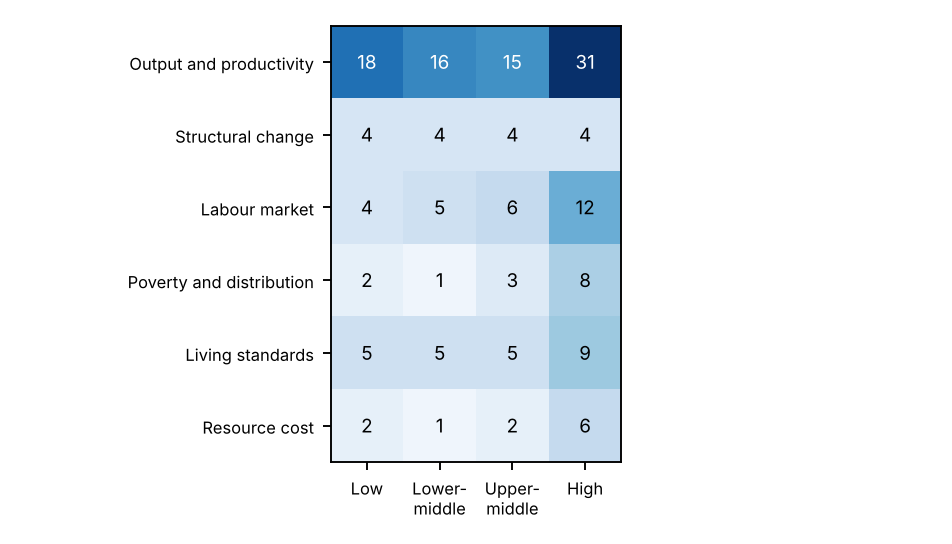
\includegraphics[width=0.58\textwidth]{fig_gap.png}
\caption{Evidence-gap map: studies per outcome family by income groups listed in the sample (a study counts in each group it lists; studies that do not state coverage are not shown).}\label{fig:gap}
\end{figure}

\subsection{A descriptive pooled association: ICT-type adoption and output}
Of 318 regression estimates in 38 studies, 148 estimates from 24 studies could be converted to partial correlations (67 reported $p$-values only, 49 were interaction terms and the rest lacked a usable number of observations or concerned crypto-assets or AI). For the 22 studies with a convertible headline estimate (Figure~\ref{fig:forest}), the random-effects pooled partial correlation is 0.161 (95\% CI 0.093 to 0.228), with $I^2 = 93\%$ and a 95\% prediction interval from $-0.144$ to 0.465. Of the headline estimates, 86\% are positive and 68\% are positive and statistically significant. A partial correlation of 0.16 corresponds to about 2.6\% of residual variance.

This figure describes the studies we found. It should not be read as an estimate of a general effect, for four reasons. First, it depends on the studies found: an earlier run with 16 studies gave 0.189 (95\% CI 0.104 to 0.274), dropping each study in turn moves it between 0.138 and 0.173, and excluding studies rated critical gives 0.146. Second, the between-study heterogeneity is very high, so a prediction interval that includes negative values describes the data better than the point estimate. Third, adjustments for small-study bias bring it down to between 0.04 and 0.09. Fourth, restricting to the 13 studies whose design includes an identification strategy beyond controls (internal or external instruments, lagged regressors or a timing design) gives a higher pooled value, 0.184 (95\% CI 0.107 to 0.261), not a lower one; since units and outcome forms differ across studies and the strategies differ in strength, we do not read this as evidence about the effect of identification. Moderator regressions (income setting, estimator, technology type) changed sign when studies were added and are not interpreted; Appendix~\ref{app:sens} reports them with the other sensitivity results so that readers can see the instability.

\begin{figure}[ht]\centering
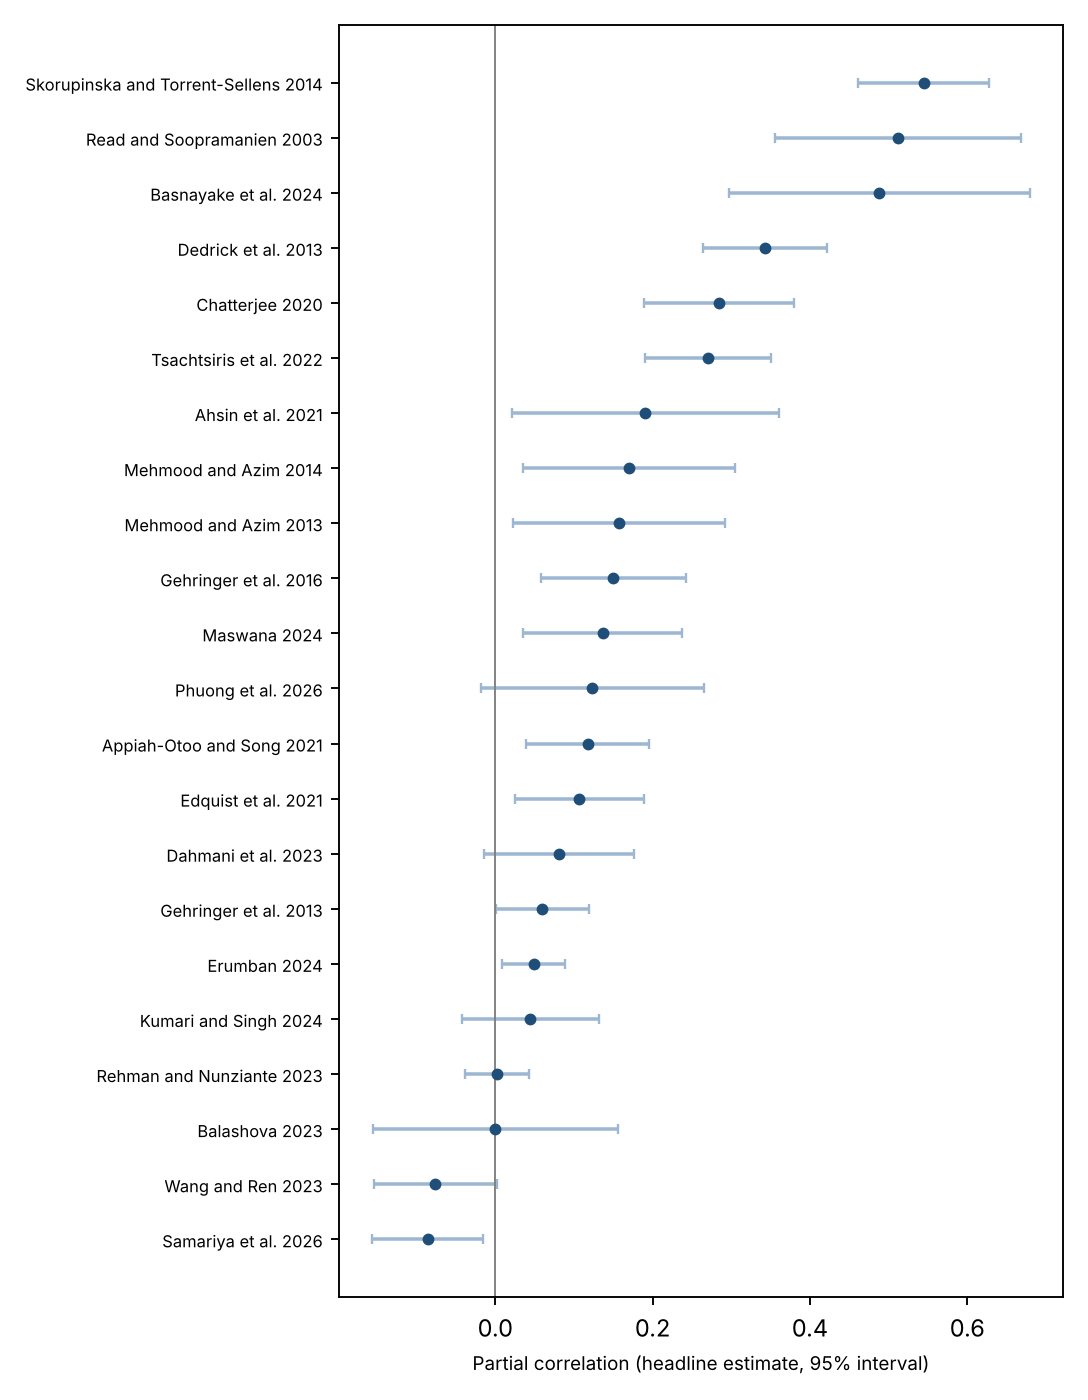
\includegraphics[width=0.62\textwidth]{fig_forest.png}
\caption{Headline partial correlations by study (95\% intervals).}\label{fig:forest}
\end{figure}

\section{Supplementary check with World Bank mobile-phone data}\label{sec:panel}
Because the included studies give conflicting answers on income differences, we checked how a simple version of the question behaves under four specifications of the same data (Appendix~\ref{app:panel} gives the design, variables and full results). Table~\ref{tab:panelshort} shows the fixed-effects panels. In the same-period specification, a 10-subscription increase in mobile adoption per 100 people goes with higher annual growth of GDP per capita in all four income groups, most clearly in lower-middle income economies (0.47 percentage points, 95\% CI 0.16 to 0.77); the low-income estimate (0.36) is imprecise (CI $-0.05$ to 0.76, 20 economies). The predetermined specification, which uses the previous period's change, does not reproduce this: it is positive only in lower-middle income economies (0.26) and negative in high-income economies ($-0.16$). The same-period associations therefore partly reflect growth driving adoption or shared shocks, and they should not be read as a payoff.

\begin{table}[ht]\centering\small
\caption{Mobile adoption and annual GDP-per-capita growth by income group: change in annual growth (percentage points) per +10 subscriptions per 100 people, five-year periods 1995--2019 (95\% CI; standard errors clustered by country).}\label{tab:panelshort}
\begin{tabular}{@{}lrrr@{}}\toprule
Income group & Economies & Same period & Previous period\\\midrule
Low & 20 & 0.36 [$-0.05$, 0.76] & $-0.38$ [$-0.86$, 0.11]\\
Lower-middle & 42 & 0.47 [0.16, 0.77] & 0.26 [0.03, 0.49]\\
Upper-middle & 51 & 0.16 [0.04, 0.28] & 0.01 [$-0.15$, 0.16]\\
High & 64 & 0.16 [0.05, 0.26] & $-0.16$ [$-0.28$, $-0.03$]\\\bottomrule
\end{tabular}\end{table}

The other two specifications give further different pictures. In a staggered event study around the year mobile subscriptions reach 10 per 100 people, with not-yet-treated economies as controls, economies that reach the threshold earlier have higher GDP per capita five years later by about 14 log points (95\% CI 0.6 to 36.5); the difference is distinguishable from zero only for high-income economies (19 log points), while the interval for low and lower-middle income economies ($-18.6$ to $+31.9$) is compatible with effects of either sign. Estimates at longer horizons mainly show that early adopters are on different growth paths and are not interpreted. Local projections show cumulative growth after a rise in adoption that is higher in lower-middle income economies (2.0 percentage points after six years) and flat or negative in the other groups. No income group shows a positive association under all four designs. We have no principled basis for preferring one design, so the check does not settle which group gains more; it shows that the answer depends on specification, which is what the included studies also suggest.

\section{Discussion}\label{sec:discussion}

\subsection{What the map shows}
Four points stand out. First, most studies that report output or productivity find a positive association with ICT-type adoption, but the sign is not uniform, the size varies strongly across studies, and the descriptive pooled partial correlation (0.16) is not stable to the studies included and shrinks under small-study adjustments. The evidence supports the statement that the association is usually positive and modest in the studies we found, and no more.

Second, authors who test conditions most often find that human capital and infrastructure raise the association, with mixed findings for governance and financial depth. This agrees with the long-run diffusion evidence that the intensity of use, rather than arrival, drives divergence \cite{comin2018}, but the studies are single-equation panels and cannot show that raising a condition would raise the return. The few thresholds that are reported, for example a human-capital index below which the effect of the digital economy is negative in Africa, each come from one study and have not been replicated.

Third, the question of whether poorer or richer economies gain more cannot be answered from this evidence. Thirty-eight studies compare income groups or regions, with nine finding larger effects in richer economies and eleven in poorer ones, and the comparisons are mostly informal and often from weak designs. Low-income economies are rarely sampled, and where they are, studies are not more likely to have weaker designs, but the number of studies is small. The lean toward larger measured gains in richer samples that an earlier version of this analysis suggested did not survive the additional studies.

Fourth, the supplementary check with World Bank data illustrates the same point from a different angle: the association between mobile adoption and growth by income group depends on the specification, and no income group is positive under all four designs. We do not take it as evidence for either group.

\subsection{AI}
The evidence on AI is too thin and too short to be put next to the evidence on earlier waves. The studies that exist, 17 in all, mostly use readiness indices, patents, robot density or occupational exposure rather than realised use, panels are short and start late, 24\% are rated critical, and only two include a low-income economy. Where they test it, they find larger measured effects in richer economies and in high-skill occupations, as for earlier technologies, but the comparison is not like for like.

\subsection{Implications}
For policy, the safest reading is that digital investment is unlikely to pay off equally everywhere and that complementary capabilities matter. The map does not support statements of the form that a given income group should expect a given payoff. Evaluations of digital programmes should report effects at several horizons, programmes in low-income settings should be monitored against the complements the literature highlights (skills, electricity, finance), and claims about AI should be treated as provisional until studies with realised-use measures and credible designs appear.

\subsection{Research agenda}
The main need is identification for developing and low-income economies, with instruments or timing designs of the kind used for submarine cables \cite{hjort2019}, and for AI, measures of realised use rather than readiness. Studies should report group-specific effects with a test of the difference, which most do not. A complete, registered, two-reviewer systematic review with Scopus, Web of Science and a full Google Scholar search would extend this map and allow inference that a pilot cannot support.

\section{Limitations}\label{sec:limits}

\begin{itemize}[leftmargin=1.4em,itemsep=2pt]
\item \textbf{Incomplete search.} The search covered OpenAlex, Crossref and NBER and the first page of four Google Scholar queries. Scopus, Web of Science and EconLit were not searched, and eleven planned Google Scholar queries were not run. Of 40 first-page Google Scholar results, 29 were missing from the main search. The map therefore describes the studies we found and is not exhaustive; any pooled figure depends on them.
\item \textbf{Single reviewer and language-model assistance.} One reviewer screened the records. A blind re-screening of a random sample gave moderate agreement at the abstract stage (79\%, kappa 0.59) and suggests that screening missed records a careful reader would include. Extraction was assisted by a language model and cross-checked by a second model run, which is not independent; the author verified the 22 estimates behind the pooled figure and checked samples of the rest, but not every extracted item has been checked by a person.
\item \textbf{Access.} Only studies with a free or supplied full text were read: about 140 of the 247 records sent to full-text assessment are unread, and paywalled studies are over-represented among them. Records from venues the author judged unreliable were skipped.
\item \textbf{Registration and grading.} The protocol was not registered before the search. The certainty of the evidence was not graded.
\item \textbf{Design quality.} No study has low risk of bias; most treat adoption as exogenous. We report associations, not causal effects. Risk-of-bias ratings are by one rater, and the cross-check disagreed with eleven of 88; the blind re-extraction agreed on the overall rating for 11 of 16 studies.
\item \textbf{Counting.} Direction counts are not weighted by size or quality and are not effect sizes. Income comparisons mix World Bank income groups, regions and developed-developing splits.
\item \textbf{Pooled figure.} It rests on 22 studies, uses an assumed number of regressors for the degrees of freedom, mixes composite indices, level and growth outcomes, and includes two studies by the same authors on the same panel. Moderator regressions changed sign as studies were added and are not interpreted.
\item \textbf{Language and period.} English only, 1995 onward.
\item \textbf{Supplementary panel check.} It gives conditional associations only. Income groups use the current World Bank classification, a planned check with initial income was not run, and CO$_2$ emissions could not be retrieved.
\end{itemize}

\section{Conclusion}\label{sec:conclusion}
This pilot evidence map of 88 cross-country studies finds that ICT-type adoption is usually associated with higher output in the studies we found, but the association is modest, very heterogeneous across studies, sensitive to which studies are included and shrinks under small-study adjustments, and it is reported to depend on human capital, infrastructure, financial depth and governance. Whether rich or poor economies gain more is not established, and the evidence on AI is too thin and too weak to compare with earlier waves. A supplementary check with World Bank data gives answers that depend on the specification. The search was incomplete and the review design had one reviewer, so the map should be read as a starting point. Credible identification for low- and middle-income economies and realised-use measures for AI are the main gaps.


\section*{Declarations}
\small
\noindent\textbf{Data and code availability.} The protocol, search and screening logs, extraction database, cross-check files, meta-regression inputs, World Bank panel and all code are in the project repository: [repository link withheld for anonymous review]. Full-text PDFs are not shared for copyright reasons.\\
\textbf{Ethics.} Not applicable; the review uses published studies and public statistics only.\\
\textbf{Author contributions (CRediT).} The review has a single author, who is responsible for all roles: conceptualisation, methodology, investigation, formal analysis, data curation, writing, supervision and project administration. The use of AI tools is described below.\\
\textbf{Conflict of interest.} The author declares no competing interests.\\
\textbf{Funding.} The author received no external funding for this work.\\
\textbf{Use of AI tools.} Generative AI tools were used to support this work: to polish the writing, to assist with screening records and extracting data from the included studies (described in the Methods), and to help write and run analysis code. The ideas, the research question and direction, and the choice of methods and algorithms are the author's own. The author reviewed the AI-assisted output and takes full responsibility for the content of this paper.\\
\textbf{Registration.} The protocol was not registered before the search (see Methods).

\normalsize
\begin{thebibliography}{99}\small
\bibitem{roller2001} L.-H. R\"oller and L. Waverman (2001). Telecommunications infrastructure and economic development: a simultaneous approach. \emph{American Economic Review} 91(4), 909--923. doi:10.1257/aer.91.4.909.
\bibitem{comin2010} D. Comin and B. Hobijn (2010). An exploration of technology diffusion. \emph{American Economic Review} 100(5), 2031--2059. doi:10.1257/aer.100.5.2031.
\bibitem{comin2018} D. Comin and M. Mestieri (2018). If technology has arrived everywhere, why has income diverged? \emph{American Economic Journal: Macroeconomics} 10(3), 137--178. doi:10.1257/mac.20150175.
\bibitem{jensen2007} R. Jensen (2007). The digital provide: information (technology), market performance, and welfare in the South Indian fisheries sector. \emph{Quarterly Journal of Economics} 122(3), 879--924. doi:10.1162/qjec.122.3.879.
\bibitem{aker2010} J. C. Aker and I. M. Mbiti (2010). Mobile phones and economic development in Africa. \emph{Journal of Economic Perspectives} 24(3), 207--232. doi:10.1257/jep.24.3.207.
\bibitem{hjort2019} J. Hjort and J. Poulsen (2019). The arrival of fast internet and employment in Africa. \emph{American Economic Review} 109(3), 1032--1079. doi:10.1257/aer.20161385.
\bibitem{autor2003} D. H. Autor, F. Levy and R. J. Murnane (2003). The skill content of recent technological change: an empirical exploration. \emph{Quarterly Journal of Economics} 118(4), 1279--1333. doi:10.1162/003355303322552801.
\bibitem{acemoglu2019} D. Acemoglu and P. Restrepo (2019). Automation and new tasks: how technology displaces and reinstates labor. \emph{Journal of Economic Perspectives} 33(2), 3--30. doi:10.1257/jep.33.2.3.
\bibitem{cohen1990} W. M. Cohen and D. A. Levinthal (1990). Absorptive capacity: a new perspective on learning and innovation. \emph{Administrative Science Quarterly} 35(1), 128--152. doi:10.2307/2393553.
\bibitem{dedrick2003} J. Dedrick, V. Gurbaxani and K. L. Kraemer (2003). Information technology and economic performance. \emph{ACM Computing Surveys} 35(1), 1--28. doi:10.1145/641865.641866.
\bibitem{prisma2020} M. J. Page et al. (2021). The PRISMA 2020 statement: an updated guideline for reporting systematic reviews. \emph{BMJ} 372, n71. doi:10.1136/bmj.n71.
\bibitem{prismap} D. Moher et al. (2015). Preferred reporting items for systematic review and meta-analysis protocols (PRISMA-P) 2015 statement. \emph{Systematic Reviews} 4, 1. doi:10.1186/2046-4053-4-1.
\bibitem{swim} M. Campbell et al. (2020). Synthesis without meta-analysis (SWiM) in systematic reviews: reporting guideline. \emph{BMJ} 368, l6890. doi:10.1136/bmj.l6890.
\bibitem{robinsi} J. A. C. Sterne et al. (2016). ROBINS-I: a tool for assessing risk of bias in non-randomised studies of interventions. \emph{BMJ} 355, i4919. doi:10.1136/bmj.i4919.
\bibitem{stanley2012} T. D. Stanley and H. Doucouliagos (2012). \emph{Meta-Regression Analysis in Economics and Business}. Routledge. doi:10.4324/9780203111710.
\bibitem{stanley2014} T. D. Stanley and H. Doucouliagos (2014). Meta-regression approximations to reduce publication selection bias. \emph{Research Synthesis Methods} 5(1), 60--78. doi:10.1002/jrsm.1095.
\bibitem{dersimonian1986} R. DerSimonian and N. Laird (1986). Meta-analysis in clinical trials. \emph{Controlled Clinical Trials} 7(3), 177--188. doi:10.1016/0197-2456(86)90046-2.
\bibitem{callaway2021} B. Callaway and P. H. C. Sant'Anna (2021). Difference-in-differences with multiple time periods. \emph{Journal of Econometrics} 225(2), 200--230. doi:10.1016/j.jeconom.2020.12.001.
\bibitem{sun2021} L. Sun and S. Abraham (2021). Estimating dynamic treatment effects in event studies with heterogeneous treatment effects. \emph{Journal of Econometrics} 225(2), 175--199. doi:10.1016/j.jeconom.2020.09.006.
\bibitem{dechaisemartin2020} C. de Chaisemartin and X. D'Haultf\oe uille (2020). Two-way fixed effects estimators with heterogeneous treatment effects. \emph{American Economic Review} 110(9), 2964--2996. doi:10.1257/aer.20181169.
\bibitem{jorda2005} \`O. Jord\`a (2005). Estimation and inference of impulse responses by local projections. \emph{American Economic Review} 95(1), 161--182. doi:10.1257/0002828053828518.
\end{thebibliography}


\appendix
\section{Included studies}\label{app:studies}
{\scriptsize
\begin{longtable}{@{}p{7.4cm} p{1.3cm} r l p{3.4cm}@{}}
\caption{Studies included in the evidence map (n = 97), in alphabetical order of the in-text citation. Technology: AI, ICT in general, mobile, internet or broadband, crypto-assets. Econ. = number of economies (n.r. = not reported). RoB = overall risk of bias (moderate, serious, critical); no study was rated low. Authors and years follow the Crossref record or, where none exists, the paper itself.}\label{tab:included}\\
\toprule Reference & Technology & Econ. & RoB & DOI \\ \midrule \endfirsthead
\toprule Reference & Technology & Econ. & RoB & DOI \\ \midrule \endhead
\bottomrule \endfoot
\textbf{Abdelhak et al. (2026)}. Abdelhak, S.; AuYong, H.N.; Li, R.Y.M.; Awal, I.M. (2026). <scp>ICT</scp>
                    Infrastructure, Economic Growth and
                    <scp>ASEAN</scp>
                    Income Heterogeneity: A Panel Analysis. \emph{Asian-Pacific Economic Literature}. & ICT, Mobile, Internet & 10 & serious & \url{https://doi.org/10.1111/apel.70056} \\
\textbf{Acheampong et al. (2022)}. Acheampong, A.O.; Opoku, E.E.O.; Dzator, J.; Kufuor, N.K. (2022). Enhancing human development in developing regions: Do ICT and transport infrastructure matter?. \emph{Technological Forecasting and Social Change}. & ICT, Mobile, Internet & 79 & serious & \url{https://doi.org/10.1016/j.techfore.2022.121725} \\
\textbf{Adamson et al. (2025)}. Adamson, A.; Fatai, ; Ajayi,  (2025). Exploring the Moderating impact of ICT Infrastructure on Trade Openness-Sectoral Growth Nexus in Sub-Saharan Africa (SSA). \emph{NIU journal of humanities.}. & ICT, Mobile, Internet & 26 & serious & \url{https://doi.org/10.58709/niujhu.v10i3.2267} \\
\textbf{Adeleye et al. (2023)}. Adeleye, B.N.; Arogundade, S.; Mduduzi, B. (2023). Empirical Analysis of Inclusive Growth, Information and Communication Technology Adoption, and Institutional Quality. \emph{Economies}. & ICT, Mobile, Internet & 193 & serious & \url{https://doi.org/10.3390/economies11040124} \\
\textbf{Adewole Adediran (2026)}. Adewole Adediran, O. (2026). Estimation of Firm Labour Productivity and Sales Growth from Artificial Intelligence in Sub-Saharan African Countries. \emph{F1000Research}. & AI & 10 & critical & \url{https://doi.org/10.12688/f1000research.179912.1} \\
\textbf{Ahsin et al. (2021)}. Ahsin, M.B.; Kueh, J.; Abdullah, M.A.b. (2021). Impact of Economic Integration and Information and Communication Technology on Economic Growth for European Union: Dynamic Panel GMM Approach. \emph{Business and Economic Research}. & ICT, Mobile, Internet & 27 & serious & \url{https://doi.org/10.5296/ber.v11i4.19064} \\
\textbf{Akpa and Asongu (2022)}. Akpa, A.; Asongu, S. (2022). The role of governance in the effect of the internet on financial inclusion in sub-Saharan Africa. \emph{SSRN Electronic Journal}. & Internet & 42 & serious & \url{https://doi.org/10.2139/ssrn.4315622} \\
\textbf{Alabi and Olaoye (2022)}. Alabi, A.W.; Olaoye, F.O. (2022). The Effect of Technology Adoption on  Financial Inclusion: A Cross-country Panel Analysis between China and Nigeria. \emph{European Journal of Business and Management Research}. & Mobile, Internet & 20 & serious & \url{https://doi.org/10.24018/ejbmr.2022.7.2.1314} \\
\textbf{Albanesi et al. (2025)}. Albanesi, S.; Dias da Silva, A.; Jimeno, J.F.; Lamo, A.; Wabitsch, A. (2025). New technologies and jobs in Europe. \emph{Economic Policy}. & AI & 16 & moderate & \url{https://doi.org/10.1093/epolic/eiae058} \\
\textbf{Alimi and Okunade (2020)}. Alimi, A.S.; Okunade, S.O. (2020). Financial Inclusion, ICT Diffusion and Poverty Reduction: Evidence from Sub-Sahara African Countries. \emph{Asian Journal of Economics and Business}. & Mobile, Internet & 27 & serious & n.a. \\
\textbf{Aly (2022)}. Aly, H. (2022). Digital transformation, development and productivity in developing countries: is artificial intelligence a curse or a blessing?. \emph{Review of Economics and Political Science}. & ICT & 25 & serious & \url{https://doi.org/10.1108/reps-11-2019-0145} \\
\textbf{Anifowose and Chummun (2025)}. Anifowose, O.; Chummun, B. (2025). A Panel Data Analysis of Determinants of Financial Inclusion in Sub-Saharan Africa (SSA) Countries from 1999 to 2024. \emph{Journal of Risk and Financial Management}. & Internet & 45 & serious & \url{https://doi.org/10.3390/jrfm18050275} \\
\textbf{Appiah-Otoo and Song (2021)}. Appiah-Otoo, I.; Song, N. (2021). The impact of ICT on economic growth-Comparing rich and poor countries. \emph{Telecommunications Policy}. & ICT, Mobile, Internet & 123 & serious & \url{https://doi.org/10.1016/j.telpol.2020.102082} \\
\textbf{Asongu and Acha-Anyi (2020)}. Asongu, S.A.; Acha-Anyi, P.N. (2020). Enhancing ICT for productivity in sub-Saharan Africa: Thresholds for complementary policies. \emph{African Journal of Science, Technology, Innovation and Development}. & Mobile, Internet & 25 & serious & \url{https://doi.org/10.1080/20421338.2020.1732596} \\
\textbf{Asongu and Agyemang-Mintah (2025)}. Asongu, S.; Agyemang-Mintah, P. (2025). The relationship between inequality and poverty in developing countries: mitigating role of virtual social network and internet access in schools. \emph{International Journal of Social Economics}. & Internet & 57 & serious & \url{https://doi.org/10.1108/ijse-09-2023-0695} \\
\textbf{Asongu and Odhiambo (2019)}. Asongu, S.A.; Odhiambo, N.M. (2019). Mobile banking usage, quality of growth, inequality and poverty in developing countries. \emph{Information Development}. & Mobile & 93 & serious & \url{https://doi.org/10.1177/0266666917744006} \\
\textbf{Asongu et al. (2021)}. Asongu, S.; Amari, M.; Jarboui, A.; Mouakher, K. (2021). ICT dynamics for gender inclusive intermediary education: minimum poverty and inequality thresholds in developing countries. \emph{SSRN Electronic Journal}. & ICT, Mobile, Internet & 57 & serious & \url{https://doi.org/10.2139/ssrn.3794050} \\
\textbf{Awad and Albaity (2024)}. Awad, A.; Albaity, M. (2024). Economic growth and the proliferation of ICT infrastructures: which causes the other?. \emph{Economic Research-Ekonomska Istraživanja}. & ICT, Mobile, Internet & 41 & serious & \url{https://doi.org/10.1080/1331677x.2024.2310100} \\
\textbf{Balashova (2023)}. Balashova, V. (2023). IMPACT OF DIGITALISATION ON PRODUCTIVITY GROWTH IN EU MEMBER STATES. \emph{Green, Blue and Digital Economy Journal}. & ICT & 27 & serious & \url{https://doi.org/10.30525/2661-5169/2023-3-2} \\
\textbf{Banga et al. (2026)}. Banga, K.; Harbansh, P.; Singh, S. (2026). Digitalisation and structural change: Evidence from cross-country analysis. \emph{Journal of Digital Economy}. & Mobile, Internet & 51 & serious & \url{https://doi.org/10.1016/j.jdec.2026.03.003} \\
\textbf{Basnayake et al. (2024)}. Basnayake, D.; Naranpanawa, A.; Selvanathan, S.; Bandara, J.S. (2024). Financial inclusion through digitalization and economic growth in Asia-Pacific countries. \emph{International Review of Financial Analysis}. & ICT, Mobile, Internet & 30 & serious & \url{https://doi.org/10.1016/j.irfa.2024.103596} \\
\textbf{Bayar et al. (2021)}. Bayar, Y.; Gavriletea, M.D.; Păun, D. (2021). IMPACT OF MOBILE PHONES AND INTERNET USE ON FINANCIAL INCLUSION: EMPIRICAL EVIDENCE FROM THE EU POST-COMMUNIST COUNTRIES. \emph{Technological and Economic Development of Economy}. & Mobile, Internet & 11 & serious & \url{https://doi.org/10.3846/tede.2021.14508} \\
\textbf{Becchetti and Adriani† (2005)}. Becchetti, L.; Adriani†, F. (2005). Does the digital divide matter? The role of information and communication technology in cross-country level and growth estimates. \emph{Economics of Innovation and New Technology}. & ICT, Mobile, Internet & 94 & serious & \url{https://doi.org/10.1080/1043859042000304043} \\
\textbf{Bello et al. (2024)}. Bello, A.A.; Hassan, A.; Akadiri, S.S.; Onuogu, I.C.; Aliyu, U.S. (2024). Towards ICT diffusion and trade liberalisation on inclusive growth in Sub-Saharan Africa. \emph{Environment, Development and Sustainability}. & ICT, Mobile, Internet & 48 & serious & \url{https://doi.org/10.1007/s10668-023-04355-x} \\
\textbf{Bergantino and Nademi (2027)}. Bergantino, A.S.; Nademi, Y. (2027). The Kuznets curve in the digital age: Understanding inequality dynamics in Europe. \emph{Telecommunications Policy}. & Internet & 28 & moderate & \url{https://doi.org/10.1016/j.telpol.2026.103354} \\
\textbf{Breemersch et al. (2019)}. Breemersch, K.; Damijan, J.P.; Konings, J. (2019). What drives labor market polarization in advanced countries? The role of China and technology. \emph{Industrial and Corporate Change}. & ICT & 19 & serious & \url{https://doi.org/10.1093/icc/dty063} \\
\textbf{Ceccobelli et al. (2012)}. Ceccobelli, M.; Gitto, S.; Mancuso, P. (2012). ICT capital and labour productivity growth: A non-parametric analysis of 14 OECD countries. \emph{Telecommunications Policy}. & ICT & 14 & serious & \url{https://doi.org/10.1016/j.telpol.2011.12.012} \\
\textbf{Chatterjee (2020)}. Chatterjee, A. (2020). Financial inclusion, information and communication technology diffusion, and economic growth: a panel data analysis. \emph{Information Technology for Development}. & ICT, Mobile, Internet & 41 & serious & \url{https://doi.org/10.1080/02681102.2020.1734770} \\
\textbf{Chinoda and Akande (2019)}. Chinoda, T.; Akande, J.O. (2019). FINANCIAL INCLUSION, MOBILE PHONE DIFFUSION, AND ECONOMIC GROWTH; EVIDENCE FROM AFRICA. \emph{International Journal of Economics and Financial Issues}. & Mobile & 32 & serious & \url{https://doi.org/10.32479/ijefi.8256} \\
\textbf{Chiplunkar and Goldberg (2022)}. Chiplunkar, G.; Goldberg, P.K. (2022). The Employment Effects of Mobile Internet in Developing Countries. \emph{}. & Mobile, Internet & 14 & moderate & \url{https://doi.org/10.3386/w30741} \\
\textbf{Dah et al. (2025)}. Dah, D.; Zahonogo, P.; Kaboré, P.F. (2025). Effects of the digital economy on economic growth in Africa: the role of human capital. \emph{Cogent Economics \&amp; Finance}. & ICT, Mobile, Internet & 41 & serious & \url{https://doi.org/10.1080/23322039.2025.2525485} \\
\textbf{Dahmani et al. (2023)}. Dahmani, M.; Mabrouki, M.; Ben Youssef, A. (2023). The ICT, financial development, energy consumption and economic growth nexus in MENA countries: dynamic panel CS-ARDL evidence. \emph{Applied Economics}. & ICT, Mobile, Internet & 11 & serious & \url{https://doi.org/10.1080/00036846.2022.2096861} \\
\textbf{Dai (2026)}. Dai, J. (2026). The nonlinear link between AI and energy poverty: Empirical evidence from global data. \emph{Journal of Cleaner Production}. & AI & 64 & serious & \url{https://doi.org/10.1016/j.jclepro.2026.148590} \\
\textbf{de la Rica and Gortazar (2016)}. de la Rica, S.; Gortazar, L. (2016). Differences in Job De-Routinization in OECD Countries: Evidence from PIAAC. \emph{}. & ICT & 22 & serious & \url{https://doi.org/10.2139/ssrn.2731999} \\
\textbf{Dedrick et al. (2013)}. Dedrick, J.; Kraemer, K.L.; Shih, E. (2013). Information Technology and Productivity in Developed and Developing Countries. \emph{Journal of Management Information Systems}. & ICT & 45 & moderate & \url{https://doi.org/10.2753/mis0742-1222300103} \\
\textbf{Drama and Senou (2025)}. Drama, B.G.H.; Senou, M.M. (2025). Unraveling the digital technologies and banking inclusion nexus in Sub Saharan Africa: What causality for what heterogeneity?. \emph{Discover Sustainability}. & Mobile, Internet & 45 & serious & \url{https://doi.org/10.1007/s43621-025-01694-9} \\
\textbf{Edquist et al. (2021)}. Edquist, H.; Goodridge, P.; Haskel, J. (2021). The Internet of Things and economic growth in a panel of countries. \emph{Economics of Innovation and New Technology}. & ICT, Mobile, Internet & 82 & serious & \url{https://doi.org/10.1080/10438599.2019.1695941} \\
\textbf{Erumban (2024)}. Erumban, A.A. (2024). Informality and aggregate labor productivity growth: Does ICT moderate the relationship?. \emph{Telecommunications Policy}. & ICT, Internet & 118 & serious & \url{https://doi.org/10.1016/j.telpol.2023.102681} \\
\textbf{Fulgenzi et al. (2024)}. Fulgenzi, R.; Gitto, S.; Mancuso, P. (2024). Information and communication technology and labour productivity growth: a production-frontier approach. \emph{Annals of Operations Research}. & ICT & 24 & serious & \url{https://doi.org/10.1007/s10479-024-05818-8} \\
\textbf{Gehringer et al. (2013)}. Gehringer, A.; Martinez-Zarzoso, I.; Nowak-Lehmann Danziger, F. (2013). The Determinants of Total Factor Productivity in the EU: Insights from Sectoral Data and Common Dynamic Processes. \emph{RePEc: Research Papers in Economics}. & ICT & 17 & serious & n.a. \\
\textbf{Gehringer et al. (2016)}. Gehringer, A.; Martínez-Zarzoso, I.; Nowak-Lehmann Danzinger, F. (2016). What are the drivers of total factor productivity in the European Union?. \emph{Economics of Innovation and New Technology}. & ICT & 17 & serious & \url{https://doi.org/10.1080/10438599.2015.1067007} \\
\textbf{Georgieff and Hyee (2022)}. Georgieff, A.; Hyee, R. (2022). Artificial Intelligence and Employment: New Cross-Country Evidence. \emph{Frontiers in Artificial Intelligence}. & AI & 23 & moderate & \url{https://doi.org/10.3389/frai.2022.832736} \\
\textbf{Gonzales (2023)}. Gonzales, J.T. (2023). Implications of AI innovation on economic growth: a panel data study. \emph{Journal of Economic Structures}. & AI & 122 & serious & \url{https://doi.org/10.1186/s40008-023-00307-w} \\
\textbf{Gopalan and Rajan (2022)}. Gopalan, S.; Rajan, R.S. (2022). Does digital financial inclusion moderate or exacerbate output volatility?. \emph{Applied Economics Letters}. & Mobile & 40 & serious & \url{https://doi.org/10.1080/13504851.2021.1963400} \\
\textbf{He and Liu (2026)}. He, X.; Liu, W. (2026). Digital transformation and income disparities: A threshold analysis in developing countries. \emph{Acta Oeconomica}. & ICT, Mobile, Internet & 45 & serious & \url{https://doi.org/10.1556/032.2025.00183} \\
\textbf{Huang et al. (2008)}. Huang, M.; Ip, W.; Yang, H.; Wang, X.; Lau, H.C. (2008). A fuzzy synthetic evaluation embedded tabu search for risk programming of virtual enterprises. \emph{International Journal of Production Economics}. & ICT & 18 & critical & \url{https://doi.org/10.1016/j.ijpe.2008.06.008} \\
\textbf{İnal et al. (2025)}. İnal, M.; Karhan, G.; Çayın, M. (2025). The Effect of Artificial Intelligence Investments on Economıc Development: Panel Data Analysis. \emph{Balkan Journal of Electrical and Computer Engineering}. & AI & 8 & serious & \url{https://doi.org/10.17694/bajece.1802500} \\
\textbf{Karaman Aksentijević et al. (2021)}. Karaman Aksentijević, N.; Ježić, Z.; Zaninović, P.A. (2021). The Effects of Information and Communication Technology (ICT) Use on Human Development—A Macroeconomic Approach. \emph{Economies}. & ICT, Mobile, Internet & 130 & serious & \url{https://doi.org/10.3390/economies9030128} \\
\textbf{Khan and Altun (2026)}. Khan, M.S.; Altun, A. (2026). AI capability and labor productivity in low- and middle-income countries: An absorptive capacity approach. \emph{Technovation}. & AI, ICT, Mobile, Internet & 63 & serious & \url{https://doi.org/10.1016/j.technovation.2026.103645} \\
\textbf{Kizi and Kizi (2025)}. Kizi, S.M.F.; Kizi, Y.M.M. (2025). Cryptocurrency Adoption Patterns and Financial Inclusion Outcomes in Emerging Market Economies. \emph{International Academic Journal of Innovative Research}. & Mobile, Internet, Crypto & 15 & critical & \url{https://doi.org/10.71086/iajir/v12i4/iajir1244} \\
\textbf{Kouladoum et al. (2022)}. Kouladoum, J.C.; Wirajing, M.A.K.; Nchofoung, T.N. (2022). Digital technologies and financial inclusion in Sub-Saharan Africa. \emph{Telecommunications Policy}. & ICT, Mobile, Internet & 43 & serious & \url{https://doi.org/10.1016/j.telpol.2022.102387} \\
\textbf{Kumari and Singh (2024)}. Kumari, R.; Singh, S.K. (2024). Impact of ICT Infrastructure, Financial Development, and Trade Openness on Economic Growth: New Evidence from Low- and High-Income Countries. \emph{Journal of the Knowledge Economy}. & ICT, Internet & 85 & serious & \url{https://doi.org/10.1007/s13132-023-01332-7} \\
\textbf{Laura Elena et al. (2024)}. Laura Elena, M.; Cristian Valeriu, P.; Mirela, D.; Tudor Gherasim, S. (2024). Artificial Intelligence Readiness and Employment: A Global Panel Analysis. \emph{ECONOMIC COMPUTATION AND ECONOMIC CYBERNETICS STUDIES AND RESEARCH}. & AI & 78 & critical & \url{https://doi.org/10.24818/18423264/58.4.24.04} \\
\textbf{Lechman and Popowska (2022)}. Lechman, E.; Popowska, M. (2022). Harnessing digital technologies for poverty reduction. Evidence for low-income and lower-middle income countries. \emph{Telecommunications Policy}. & Mobile, Internet & 40 & serious & \url{https://doi.org/10.1016/j.telpol.2022.102313} \\
\textbf{Lee (2025)}. Lee, K.F. (2025). Artificial Intelligence and Labour Markets in Southeast Asia: An Empirical Examination. \emph{Asian Economics Letters}. & AI & 1 & serious & \url{https://doi.org/10.46557/001c.132415} \\
\textbf{Leila (2024)}. Leila, B.L. (2024). IMPACT OF ICT ON ECONOMIC GROWTH: CASE OF OECD AND MENA COUNTRIES. \emph{Interciencia}. & ICT, Mobile, Internet & 32 & serious & \url{https://doi.org/10.59671/dga69} \\
\textbf{Maswana (2024)}. Maswana, J.C. (2024). Exploring the growth effects of Artificial Intelligence in developing countries in Africa using a semi-endogenous growth model. \emph{AEA/ASSA conference paper}. & AI, ICT & 48 & critical & n.a. \\
\textbf{Mehar (2023)}. Mehar, M.A. (2023). Digital Divide, Credit Financing and Financial Inclusion: Changing Patterns of Poverty, Employment and Income Inequalities. \emph{DergiPark (Istanbul University)}. & Mobile, Internet & 148 & serious & n.a. \\
\textbf{Mehmood and Azim (2013)}. Mehmood, B.; Azim, P. (2013). Does ICT Participate in Economic Convergence among Asian Countries: Evidence from Dynamic Panel Data Model. \emph{Informatica Economica}. & ICT, Mobile, Internet & 24 & serious & \url{https://doi.org/10.12948/issn14531305/17.2.2013.01} \\
\textbf{Mehmood and Azim (2014)}. Mehmood, B.; Azim, P. (2014). Total Factor Productivity, Demographic Traits and ICT: Empirical Analysis for Asia. \emph{Informatica Economica}. & ICT, Mobile, Internet & 24 & serious & \url{https://doi.org/10.12948/issn14531305/18.1.2014.01} \\
\textbf{Mensah (2023)}. Mensah, J.T. (2023). Mobile Phones and Local Economic Development: A Global Evidence. \emph{}. & Mobile, Internet & 120 & moderate & \url{https://doi.org/10.1596/1813-9450-10526} \\
\textbf{Mialon and Nesson (2020)}. Mialon, H.M.; Nesson, E.T. (2020). THE ASSOCIATION BETWEEN MOBILE PHONES AND THE RISK OF BRAIN CANCER MORTALITY: A 25-YEAR CROSS-COUNTRY ANALYSIS. \emph{Contemporary Economic Policy}. & Mobile & 88 & serious & \url{https://doi.org/10.1111/coep.12456} \\
\textbf{Molinari and Torres (2018)}. Molinari, B.; Torres, J.L. (2018). TECHNOLOGICAL SOURCES OF ECONOMIC GROWTH IN EUROPE AND THE U.S.. \emph{Technological and Economic Development of Economy}. & ICT & 10 & serious & \url{https://doi.org/10.3846/20294913.2017.1280557} \\
\textbf{Moolio et al. (2026)}. Moolio, P.; Haque, M.J.; Uddin, K.M.N.; Tan, K.G.; Liew, C.P. (2026). The Digital Maturity Paradox: The Divergent Impact of Network Readiness and FDI Across Development Tiers. \emph{Economies}. & ICT & 121 & critical & \url{https://doi.org/10.3390/economies14080320} \\
\textbf{Mourad and Gül (2025)}. Mourad, Z.; Gül, M. (2025). Crypto-driven growth: A comparative study of Bitcoin and Ethereum on economic growth for multi-country analysis. \emph{Russian Journal of Economics}. & Crypto & 14 & critical & \url{https://doi.org/10.32609/j.ruje.11.164511} \\
\textbf{Nawaz (2026)}. Nawaz, S. (2026). Impact of Generative AI Adoption on Micro and Small Enterprises in Emerging Economies. \emph{International Journal of Progress in Social Sciences Development}. & Other & 3 & critical & \url{https://doi.org/10.64060/ijpssdv2i12} \\
\textbf{Nguyen and Duong (2026)}. Nguyen, T.P.; Duong, T.T.T. (2026). Artificial intelligence investment and renewable energy for environmental sustainability in ASEAN-5 under the foreign direct investment threshold. \emph{Discover Sustainability}. & AI & 5 & serious & \url{https://doi.org/10.1007/s43621-026-03998-w} \\
\textbf{Olutimehin et al. (2026)}. Olutimehin, A.T.; Olaniyi, O.M.; Alao, A.I.; Olaniyi, O.O.; Adesokan, O.Z. (2026). The Economic Value of Agentic AI: A Comparative Analysis of Its Impact on Growth and Business Productivity in Developed and Emerging Economies. \emph{Asian Journal of Research in Computer Science}. & AI & 10 & critical & \url{https://doi.org/10.9734/ajrcos/2026/v19i5859} \\
\textbf{Phuong et al. (2026)}. Phuong, V.M.; Giang, N.T.; Anh, L.T. (2026). Twin Transition and Labor Informality in Asia-Pacific: Threshold Effects and Income-Group Heterogeneity. \emph{Economies}. & ICT, Internet & 17 & serious & \url{https://doi.org/10.3390/economies14090398} \\
\textbf{Read and Soopramanien (2003)}. Read, R.; Soopramanien, D. (2003). Bridging the digital divide: the growth implications of e-commerce for small and developing states. \emph{RePEc: Research Papers in Economics}. & Internet & 205 & critical & n.a. \\
\textbf{Rehman and Nunziante (2023)}. Rehman, N.U.; Nunziante, G. (2023). The effect of the digital economy on total factor productivity in European regions. \emph{Telecommunications Policy}. & ICT, Internet & 27 & serious & \url{https://doi.org/10.1016/j.telpol.2023.102650} \\
\textbf{Richmond and Triplett (2018)}. Richmond, K.; Triplett, R.E. (2018). ICT and income inequality: a cross-national perspective. \emph{International Review of Applied Economics}. & Mobile, Internet & 109 & serious & \url{https://doi.org/10.1080/02692171.2017.1338677} \\
\textbf{Saba (2025)}. Saba, C.S. (2025). Artificial intelligence (AI)-poverty-economic growth nexus in selected BRICS-Plus countries: does the moderating role of governance matter?. \emph{AI \&amp; SOCIETY}. & AI & 5 & serious & \url{https://doi.org/10.1007/s00146-025-02213-0} \\
\textbf{Saba and Ngepah (2022)}. Saba, C.S.; Ngepah, N. (2022). ICT Diffusion, Industrialisation and Economic Growth Nexus: an International Cross-country Analysis. \emph{Journal of the Knowledge Economy}. & ICT, Mobile, Internet & 171 & serious & \url{https://doi.org/10.1007/s13132-021-00795-w} \\
\textbf{Saba et al. (2024)}. Saba, C.S.; Ngepah, N.; Odhiambo, N.M. (2024). Information and Communication Technology (ICT), Growth and Development in Developing Regions: Evidence from a Comparative Analysis and a New Approach. \emph{Journal of the Knowledge Economy}. & ICT, Mobile, Internet & 73 & serious & \url{https://doi.org/10.1007/s13132-023-01571-8} \\
\textbf{Samariya et al. (2026)}. Samariya, A.K.; Bahl, S.; Sharma, D. (2026). Internet and Economic Growth Across Income Levels: a Panel Data Analysis. \emph{Journal of the Knowledge Economy}. & Internet & 78 & serious & \url{https://doi.org/10.1007/s13132-026-03136-x} \\
\textbf{Santos et al. (2023)}. Santos, A.M.; Barbero, J.; Salotti, S.; Conte, A. (2023). Job creation and destruction in the digital age: Assessing heterogeneous effects across European Union countries. \emph{Economic Modelling}. & ICT & 27 & moderate & \url{https://doi.org/10.1016/j.econmod.2023.106405} \\
\textbf{Satrianto and Ikhsan (2023)}. Satrianto, A.; Ikhsan, A. (2023). The effect of information and communication technology on economic growth high-income countries. \emph{Asian Economic and Financial Review}. & ICT, Mobile, Internet & 10 & serious & \url{https://doi.org/10.55493/5002.v13i9.4824} \\
\textbf{Shah and Krishnan (2024)}. Shah, C.S.; Krishnan, S. (2024). ICT, Gender Inequality, and Income Inequality: A Panel Data Analysis Across Countries. \emph{Information Systems Frontiers}. & ICT, Mobile, Internet & 86 & serious & \url{https://doi.org/10.1007/s10796-023-10396-4} \\
\textbf{Sharma et al. (2021)}. Sharma, G.D.; Rahman, M.M.; Jain, M.; Chopra, R. (2021). Nexus between energy consumption, information and communications technology, and economic growth: An enquiry into emerging Asian countries. \emph{Journal of Public Affairs}. & ICT, Mobile, Internet & 10 & serious & \url{https://doi.org/10.1002/pa.2172} \\
\textbf{Skorupinska and Torrent-Sellens (2014)}. Skorupinska, A.A.; Torrent-Sellens, J. (2014). The Role of ICT in the Productivity of Central and Eastern European Countries: Cross-country Comparison. \emph{Revista de Economía Mundial}. & ICT, Internet & 21 & serious & \url{https://doi.org/10.33776/rem.v0i39.3987} \\
\textbf{Sultanova and Naser (2026)}. Sultanova, G.; Naser, H. (2026). The impact of information and communication technologies on export diversification: Evidence from developing countries. \emph{The Journal of International Trade \&amp; Economic Development}. & ICT, Mobile, Internet & 110 & moderate & \url{https://doi.org/10.1080/09638199.2024.2419406} \\
\textbf{Sze-Wei Yong et al. (2024)}. Sze-Wei Yong, ; Siong-Hook Law, ; Saifuzzaman Ibrahim, ; Wan Norhidayah W Mohamad,  (2024). Icts And Labour Productivity Nexus In Developing Countries: Evidence From Panel Estimation Approach. \emph{International Journal of Business and Society}. & ICT, Mobile, Internet & 84 & serious & \url{https://doi.org/10.33736/ijbs.6868.2024} \\
\textbf{Taniguchi and Yamada (2020)}. Taniguchi, H.; Yamada, K. (2020). The Race between Technological Progress and Female Advancement: Changes in Gender and Skill Premia in OECD Countries. \emph{arXiv (Cornell University)}. & ICT & 11 & moderate & n.a. \\
\textbf{Taniguchi and Yamada (2022)}. Taniguchi, H.; Yamada, K. (2022). ICT capital–skill complementarity and wage inequality: Evidence from OECD countries. \emph{Labour Economics}. & ICT & 14 & moderate & \url{https://doi.org/10.1016/j.labeco.2022.102151} \\
\textbf{Tian and Zhang (2025)}. Tian, J.; Zhang, Y. (2025). Does artificial intelligence help in improving human capital based educational development? Evidence from 29 countries. \emph{Technology in Society}. & AI & 29 & serious & \url{https://doi.org/10.1016/j.techsoc.2025.103004} \\
\textbf{Tsachtsiris et al. (2022)}. Tsachtsiris, G.; Magoutas, A.; Papadogonas, T. (2022). ICT and Economic Growth in EU: A macro Level Comparison of Estimated ICT Output Elasticities. \emph{Journal of Global Information Technology Management}. & ICT & 27 & moderate & \url{https://doi.org/10.1080/1097198x.2022.2094182} \\
\textbf{Tunçsiper (2025)}. Tunçsiper, Ç. (2025). From Digital Divide to Employment Equity: How Digitalization Affects Women's Involvement in the Workforce in OECD Countries. \emph{Multidisciplinary Journal of Gender Studies}. & Mobile, Internet & 22 & critical & \url{https://doi.org/10.17583/generos.15672} \\
\textbf{Wang and Ren (2023)}. Wang, A.; Ren, J. (2023). The impact of the digital economy on green total factor productivity in Belt and Road countries: the mediating role of energy transition. \emph{Frontiers in Environmental Science}. & ICT, Internet & 40 & serious & \url{https://doi.org/10.3389/fenvs.2023.1213961} \\
\textbf{Wang and Shen (2024)}. Wang, F.; Shen, S. (2024). Does the digital economy development improve or exacerbate income inequality? International evidence. \emph{Managerial and Decision Economics}. & ICT, Mobile, Internet & 97 & serious & \url{https://doi.org/10.1002/mde.4231} \\
\textbf{Wang et al. (2025)}. Wang, Q.; Li, Y.; Pata, U.K.; Li, R. (2025). Artificial intelligence and global carbon inequality: Addressing the challenges and opportunities for SDG 10, SDG 12, and SDG 13. \emph{Geoscience Frontiers}. & AI & 67 & serious & \url{https://doi.org/10.1016/j.gsf.2025.102072} \\
\textbf{Yin and Choi (2023)}. Yin, Z.H.; Choi, C.H. (2023). Does digitalization contribute to lesser income inequality? Evidence from G20 countries. \emph{Information Technology for Development}. & Mobile, Internet & 19 & serious & \url{https://doi.org/10.1080/02681102.2022.2123443} \\
\textbf{Yu and Liu (2024)}. Yu, H.; Liu, H. (2024). Impact of digitization on carbon productivity: an empirical analysis of 136 countries. \emph{Scientific Reports}. & Mobile, Internet & 136 & serious & \url{https://doi.org/10.1038/s41598-024-55848-2} \\
\textbf{Zelenyuk (2005)}. Zelenyuk, V. (2005). Testing the impact of ICT in developed countries during 1980-1995: distributional analysis in Solow’s growth accounting framework. \emph{RePEc: Research Papers in Economics}. & ICT & 15 & serious & n.a. \\
\textbf{Zhang and Totouom (2026)}. Zhang, G.; Totouom, A. (2026). Reducing Gender Inequality in Education in Developing Countries: Do Information and Communication Technologies Matter?. \emph{Sustainable Development}. & ICT, Mobile, Internet & 64 & serious & \url{https://doi.org/10.1002/sd.71201} \\
\textbf{Çetin and Kutlu (2025)}. Çetin, C.N.; Kutlu, E. (2025). The Impact of Artificial Intelligence on Employment: A Panel Data Analysis for Selected Countries. \emph{Ekonomi Politika ve Finans Arastirmalari Dergisi}. & AI & 29 & serious & \url{https://doi.org/10.30784/epfad.1621455} \\
\textbf{Özocaklı (2026)}. Özocaklı, D. (2026). Can Artificial Intelligence Drive Sustainable Growth? Empirical Evidence on the AI–Energy–Growth Nexus in Advanced Economies. \emph{Sustainability}. & AI, ICT & 9 & serious & \url{https://doi.org/10.3390/su18052308} \\
\end{longtable}
}
{\scriptsize
\begin{longtable}{@{}p{7.4cm} p{1.3cm} r l p{3.4cm}@{}}
\caption{Studies added by the supplementary searches for the analysis of income contrasts (n = 67). Columns as in Table~\ref{tab:included}.}\label{tab:included2}\\
\toprule Reference & Technology & Econ. & RoB & DOI \\ \midrule \endfirsthead
\toprule Reference & Technology & Econ. & RoB & DOI \\ \midrule \endhead
\bottomrule \endfoot
\textbf{Adeleye et al. (2023b)}. Adeleye, B.N.; Achugamonu, B.U.; George, T.O.; Ogbari, M.E.; Ola-David, O. (2023). ICT Leapfrogging Amidst Labour Force-Economic Growth Nexus in EAP and ECA Regions. \emph{Scientific Annals of Economics and Business 70(1), 17-40}. & Mobile, Internet & 81 & serious & \url{https://doi.org/10.47743/saeb-2023-0004} \\
\textbf{Afzal et al. (2022)}. Afzal, A.; Firdousi, S.F.; Waqar, A.; Awais, M. (2022). The Influence of Internet Penetration on Poverty and Income Inequality. \emph{SAGE Open 12(3)}. & Mobile, Internet & 86 & serious & \url{https://doi.org/10.1177/21582440221116104} \\
\textbf{Ahsen (2025)}. Ahsen, A. (2025). Assessing Environmental Impacts of ICT integration in Asian Economies. \emph{Pakistan Journal of Economic Studies (PJES)}. & ICT, Mobile, Internet & n.r. & serious & n.a. \\
\textbf{Albiman and Sulong (2017)}. Albiman, M.M.; Sulong, Z. (2017). The linear and non-linear impacts of ICT on economic growth, of disaggregate income groups within SSA region. \emph{Telecommunications Policy 41(7-8), 555-572}. & ICT, Mobile, Internet & 45 & serious & \url{https://doi.org/10.1016/j.telpol.2017.07.007} \\
\textbf{Alghamdi et al. (2026)}. Alghamdi, R.; Elimam, H.; Bardesi, H.J. (2026). ICT Diffusion and Labor Productivity in G20 Countries: Development-Stage Differences and Granger Evidence. \emph{European Journal of Sustainable Development 15(2), 208-208}. & Internet & 19 & moderate & \url{https://doi.org/10.14207/ejsd.2026.v15n2p208} \\
\textbf{Aslam et al. (2020)}. Aslam, A.; Naveed, A.; Shabbir, G. (2020). Is it an institution, digital or social inclusion that matters for inclusive growth? A panel data analysis. \emph{Quality \& Quantity 55(1), 333-355}. & ICT, Mobile, Internet & 83 & serious & \url{https://doi.org/10.1007/s11135-020-01008-3} \\
\textbf{Assaaoudi (2026)}. Assaaoudi, A. (2026). Internet Use, Socioeconomic Indicators, and Suicide Mortality: An Ecological Analysis. \emph{University of Ottawa Science Undergraduate Research Journal 5(1)}. & Internet & n.r. & serious & \url{https://doi.org/10.18192/osurj.v5i1.8034} \\
\textbf{Azam et al. (2023)}. Azam, M.; Ameur, H.B.; Ftiti, Z.; Hunjra, A.I.; Louhichi, W. (2023). The Role of ICTs on Innovation Process of Environment and Energy Convergence. \emph{IEEE Transactions on Engineering Management 71, 4418-4440}. & ICT, Mobile, Internet & 60 & serious & \url{https://doi.org/10.1109/tem.2022.3233785} \\
\textbf{Bala (2024)}. Bala, P. (2024). The Impact of Mobile Broadband and Internet Bandwidth on Human Development—A Comparative Analysis of Developing and Developed Countries. \emph{Journal of the Knowledge Economy 15(4), 16419-16453}. & Mobile, Internet & 180 & moderate & \url{https://doi.org/10.1007/s13132-023-01711-0} \\
\textbf{Bankole et al. (2011)}. Bankole, F.O.; Shirazi, F.; Brown, I. (2011). Investigating the Impact of ICT Investments on Human Development. \emph{The Electronic Journal of Information Systems in Developing Countries 48(1), 1-19}. & ICT & 51 & serious & \url{https://doi.org/10.1002/j.1681-4835.2011.tb00344.x} \\
\textbf{Barcia et al. (2026)}. Barcia, M.M.C.; Córdoba, É.F.; Barcia, L.A.C.; Loor, F.O.C.; Cedeño, P.R.F.; Alava, L.A.R. (2026). Digital Connectivity, Access Infrastructure, and the Global Expansion of Higher Education. \emph{International Journal of Computer Information Systems and Industrial Management Applications 18(7s), 607-615}. & Mobile, Internet & 163 & serious & \url{https://doi.org/10.70917/ijcisim-2026-3119} \\
\textbf{Bilal et al. (2024)}. Bilal, M.; Aqib, S.; Raza, A. (2024). Strengthening economic resilience through ICT during the COVID-19 pandemic: evidence from 100 countries. \emph{Discover Sustainability 5(1)}. & ICT, Mobile, Internet & 100 & serious & \url{https://doi.org/10.1007/s43621-024-00729-x} \\
\textbf{Danish et al. (2019)}. Danish, ; Zhang, J.; Wang, B.; Latif, Z. (2019). Towards cross-regional sustainable development: The nexus between information and communication technology, energy consumption, and CO 2 emissions. \emph{Sustainable Development 27(5), 990-1000}. & ICT, Mobile & 73 & serious & \url{https://doi.org/10.1002/sd.2000} \\
\textbf{Dewan and Kraemer (2000)}. Dewan, S.; Kraemer, K.L. (2000). Information Technology and Productivity: Evidence from Country-Level Data. \emph{Management Science 46(4), 548-562}. & Other & 36 & serious & \url{https://doi.org/10.1287/mnsc.46.4.548.12057} \\
\textbf{Dong and Xu (2025)}. Dong, Y.; Xu, Q. (2025). How does digital economy achieve inclusive economic growth with efficiency, equity and green? International evidence. \emph{Management of Environmental Quality An International Journal 36(5), 1283-1303}. & ICT & 98 & serious & \url{https://doi.org/10.1108/meq-07-2024-0284} \\
\textbf{Duan et al. (2026)}. Duan, L.; Chen, Y.; He, Y.; Kong, W.; Wei, M. (2026). Is digital economy development conducive to fostering innovation chain industry convergence? Empirical evidence from global cross-country studies. \emph{Journal of Digital Intelligence and Economic Growth 3(3)}. & ICT & 53 & serious & \url{https://doi.org/10.63768/jdieg.v3i3.002} \\
\textbf{Durusoy (2024)}. Durusoy, Ö.T. (2024). DİGİTAL EKONOMİK GELİŞMENİN TARIM SEKTÖRÜ KARBON EMİSYON YOĞUNLUĞU ÜZERİNDEKİ ETKİLERİ : GELİŞMİŞ VE GELİŞMEKTE OLAN ÜLKELERDE PANEL VERİ ANALİZİ. \emph{3 SEKTÖR SOSYAL EKONOMİ DERGİSİ}. & Internet & 16 & serious & \url{https://doi.org/10.15659/3.sektor-sosyal-ekonomi.24.09.2492} \\
\textbf{Edquist (2022)}. Edquist, H.O. (2022). The economic impact of mobile broadband speed. \emph{Telecommunications Policy 46(5), 102351-102351}. & Mobile, Internet & 116 & moderate & \url{https://doi.org/10.1016/j.telpol.2022.102351} \\
\textbf{Farhadi et al. (2012)}. Farhadi, M.; Ismail, R.; Fooladi, M. (2012). Information and Communication Technology Use and Economic Growth. \emph{PLoS ONE 7(11), e48903-e48903}. & ICT, Mobile, Internet & 159 & serious & \url{https://doi.org/10.1371/journal.pone.0048903} \\
\textbf{Ganić (2024)}. Ganić, M. (2024). Digitalization-growth nexus: some empirical evidence from four regions with a Muslim majority. \emph{Pressacademia}. & ICT & 48 & serious & \url{https://doi.org/10.17261/pressacademia.2023.1860} \\
\textbf{Gul et al. (2020)}. Gul, F.; Majeed, M.T.; Ahmad, I.; Lorestani, V.Z.; Meyer, D.; Máté, D. (2020). THE NEXUS OF E-GOVERNMENT AND INCREASED PRODUCTIVITY RELATIVE TO INCOME LEVEL COMPARISON. \emph{Business Management and Education 18(1), 88-105}. & Other & 168 & serious & \url{https://doi.org/10.3846/bme.2020.12067} \\
\textbf{Gulalai et al. (2026)}. Gulalai, ; Kanval, N.; Bashir, S.; Makin, F.; Anjum, U.; Shabbır, M.S.e.a. (2026). THE FINANCE–DIGITALIZATION–PRODUCTIVITY NEXUS: NEW EVIDENCE FROM DEVELOPING AND HIGH-INCOME ECONOMIES. \emph{Acta Innovations 64(3s)}. & ICT & 187 & serious & \url{https://doi.org/10.62441/actainnovations.vi.3669} \\
\textbf{H.P.B. (2026)}. H.P.B., K. (2026). The Global AI Divide: A Cross-National Analysis of Artificial Intelligence Integration and Labor Market Inequality. \emph{Journal of Eurasian Social Sciences 1(2), 221-237}. & AI & 95 & serious & \url{https://doi.org/10.68283/jess.v1.i2.a23} \\
\textbf{Hamka (2025)}. Hamka, H. (2025). Globalization And Digital Transformation As Demographic And Green Economic Policies In Southeast Asia. \emph{Journal of Engineering and Science Application. 2(1), 61-70}. & ICT & 82 & critical & \url{https://doi.org/10.69693/jesa.v2i1.23} \\
\textbf{Haq et al. (2026)}. Haq, I.u.; Andleeb, S.; Manzoor, T.; Habib, Z. (2026). The Economic Impact of Artificial Intelligence and Digital Transformation on Employment, Productivity, and Sustainable Growth. \emph{ACADEMIA International Journal for Social Sciences 5(3(s8)), 287-313}. & AI, ICT & 85 & serious & \url{https://doi.org/10.63056/academia.5.3(s8).2026.2111} \\
\textbf{Hcine et al. (2026)}. Hcine, A.; Zarrad, O.; Helali, K. (2026). Impacts of the digital economy on industrial employment and CO2 emissions: a comparison between developed and developing countries. \emph{Journal of Economic Structures 15(1)}. & ICT & 15 & critical & \url{https://doi.org/10.1186/s40008-026-00384-7} \\
\textbf{Hoz-Rosales et al. (2019)}. Hoz-Rosales, B.d.l.; Ballesta, J.A.C.; Tamayo-Torres, I.; Buelvas-Ferreira, K. (2019). Effects of Information and Communication Technology Usage by Individuals, Businesses, and Government on Human Development: An International Analysis. \emph{IEEE Access 7, 129225-129243}. & ICT & 145 & serious & \url{https://doi.org/10.1109/access.2019.2939404} \\
\textbf{Hu (2025)}. Hu, Y. (2025). The Impact of the Digital Economy on Employment at High Skill Levels—Panel Analysis Based on the 82 Countries. \emph{Operations Research and Fuzziology 15(02), 792-804}. & ICT & 82 & serious & \url{https://doi.org/10.12677/orf.2025.152126} \\
\textbf{Iqbal et al. (2026)}. Iqbal, M.A.B.; Aftab, M.U.; Shaukat, S. (2026). The Digital Divide And The Great Divergence: Internet Penetration, Economic Growth, And Income Inequality In A Panel Of 58 Countries (2000–2022). \emph{Advance Journal of Econometrics and Finance}. & Internet & 58 & serious & \url{https://doi.org/10.63075/hxaqhf53} \\
\textbf{Irfan et al. (2026)}. Irfan, M.; Khan, W.; Kandhro, A.B.; Shan-e-Zehra,  (2026). The Impact of Digital Financial Inclusion on Economic Growth: Evidence from Developing Economies. \emph{ACADEMIA International Journal for Social Sciences 5(3(s5)), 323-363}. & ICT, Mobile & 67 & serious & \url{https://doi.org/10.63056/academia.5.3(s5).2026.1978} \\
\textbf{Kasap and Ülger (2025)}. Kasap, A.; Ülger, M. (2025). The Effects of Digitalization on Economic Growth: A Comparative Panel Data Analysis of EU and BRICS-T Countries. \emph{Dynamics in Social Sciences and Humanities 6(1), 10-24}. & Mobile, Internet & n.r. & serious & \url{https://doi.org/10.62425/dssh.1623503} \\
\textbf{Kočišová and Petriková (2025)}. Kočišová, K.; Petriková, T. (2025). Can Digitalisation Mitigate Financial Exclusion? Investigation of Regional Disparities. \emph{Journal of Central Banking Theory and Practice 14(3), 79-104}. & Internet & 123 & serious & \url{https://doi.org/10.2478/jcbtp-2025-0024} \\
\textbf{Let et al. (2018)}. Let, H.S.; Hamzah, H.Z.; ZulkornainYusop, ; Mazlan, N.S. (2018). ICT Adoption Drives Productivity in Developed and Developing Countries. \emph{Jurnal Ekonomi Malaysia 52(3)}. & Mobile, Internet & 89 & serious & \url{https://doi.org/10.17576/jem-2018-5203-16} \\
\textbf{Li et al. (2024)}. Li, Y.; Li, X.; Wang, X.; Feng, C.Q. (2024). SUSTAINABLE DIGITAL TRANSFORMATION: THE NEXUS BETWEEN ICT AND GLOBAL GREEN ECONOMIC GROWTH. \emph{Technological and Economic Development of Economy 30(5), 1275-1305}. & ICT & 65 & moderate & \url{https://doi.org/10.3846/tede.2024.21050} \\
\textbf{Liu (2026)}. Liu, Y. (2026). The Impact of Digital Divide on Income Inequality—from The Perspective of Industrial Structure. \emph{Journal of innovation and development 14(3), 384-391}. & Mobile & 142 & critical & \url{https://doi.org/10.54097/rywgy010} \\
\textbf{Liu et al. (2023)}. Liu, K.; Feng, Z.; Zhang, Q. (2023). Examining the role of digitalization and gig economy in achieving a low carbon society: an empirical study across nations. \emph{Frontiers in Environmental Science 11}. & Internet & n.r. & serious & \url{https://doi.org/10.3389/fenvs.2023.1197708} \\
\textbf{Ma (2025)}. Ma, Q. (2025). The Promoting Role of Digital Infrastructure Construction on Local Economic Development: Evidence from Belt and Road Countries. \emph{Finance and Trade Dynamics 1(2), 1-12}. & ICT & 65 & serious & \url{https://doi.org/10.63808/ftd.v1i2.63} \\
\textbf{Mahdavi and Sojoodi (2021)}. Mahdavi, S.; Sojoodi, S. (2021). Impact of ICT on Environment. \emph{Research Square}. & ICT & 30 & serious & \url{https://doi.org/10.21203/rs.3.rs-1020622/v1} \\
\textbf{Majeed (2018)}. Majeed, M.T. (2018). Information and communication technology (ICT) and environmental sustainability: A comparative empirical analysis. \emph{Pakistan Journal of Commerce and Social Sciences 12(3), 758-783}. & ICT, Internet & 132 & serious & n.a. \\
\textbf{Majeed and Ayub (2018)}. Majeed, M.T.; Ayub, T. (2018). Information and communication technology (ICT) and economic growth nexus: A comparative global analysis. \emph{Pakistan Journal of Commerce and Social Sciences 12(2), 443-476}. & ICT, Mobile, Internet & 149 & serious & n.a. \\
\textbf{Milindi and Inglesi-Lotz (2022)}. Milindi, C.B.; Inglesi-Lotz, R. (2022). Impact of technological progress on carbon emissions in different country income groups. \emph{Energy \& Environment 34(5), 1348-1382}. & ICT, Mobile, Internet & 60 & serious & \url{https://doi.org/10.1177/0958305x221087507} \\
\textbf{Mukhtar et al. (2025)}. Mukhtar, M.A.; Nasreen, F.; Rani, Z. (2025). The Impact of Remittances, Financial Infrastructure, Internet Usage, and Taxation on Gross Domestic Product. \emph{Journal of Social Signs Review}. & Internet & 81 & serious & n.a. \\
\textbf{Nguyen (2022)}. Nguyen, V.B. (2022). Does Digitalization Widen Income Inequality? A Comparative Assessment for Advanced and Developing Economies. \emph{South East European Journal of Economics and Business 17(2), 154-171}. & ICT, Internet & 65 & serious & \url{https://doi.org/10.2478/jeb-2022-0021} \\
\textbf{Nguyen (2023)}. Nguyen, V.B. (2023). The role of digitalization in the FDI – income inequality relationship in developed and developing countries. \emph{Journal of Economics Finance and Administrative Science 28(55), 6-26}. & ICT, Internet & 65 & serious & \url{https://doi.org/10.1108/jefas-09-2021-0189} \\
\textbf{Ozili (2026)}. Ozili, P.K. (2026). Artificial intelligence (AI) innovation and economic growth: asymmetric analysis and role of stock market, financial stability and trade openness. \emph{Journal of Economic Studies, 1-19}. & AI & 50 & serious & \url{https://doi.org/10.1108/jes-02-2026-0176} \\
\textbf{Parveen et al. (2023)}. Parveen, A.; Mehmood, K.; Javed, M. (2023). Assessing the Impact of ICT, Tourism, Globalization and Urbanization on Environmental Degradation and Economic Growth. \emph{NUML International Journal of Business \& Management 18(2)}. & ICT & 65 & serious & \url{https://doi.org/10.52015/nijbm.v18i2.173} \\
\textbf{Pasha (2025)}. Pasha, S. (2025). Impact of digitalization on sustainable development amidst geopolitical risks. \emph{International journal of applied research 11(11S), 133-136}. & ICT & n.r. & critical & \url{https://doi.org/10.22271/allresearch.2025.v11.i11sa.13060} \\
\textbf{Perveen and Majeed (2024)}. Perveen, S.; Majeed, M.T. (2024). Analyzing the Influence of Digitalization on Income Inequality: A Comparative Analysis of Developed and Developing Economies. \emph{Social science multidisciplinary review}. & ICT, Mobile, Internet & 127 & moderate & n.a. \\
\textbf{Pham et al. (2025)}. Pham, N.T.; Vo, T.H.; Huynh, L.G.; Nguyen, M.H. (2025). The impact of digital transformation on economic growth: A global evidence. \emph{Journal of Finance - Marketing Research 4(1en), 19-33}. & ICT, Mobile, Internet & 77 & serious & \url{https://doi.org/10.52932/jfmr.v4i1en.738} \\
\textbf{Pradhan et al. (2022)}. Pradhan, R.P.; Arvin, M.B.; Nair, M.S.; Hall, J.H.; Bennett, S.E. (2022). Institutional development in an information-driven economy: can ICTs enhance economic growth for low- and lower middle-income countries?. \emph{Information Technology for Development 28(3), 468-487}. & ICT, Mobile, Internet & 79 & serious & \url{https://doi.org/10.1080/02681102.2022.2051417} \\
\textbf{Pérez et al. (2026)}. Pérez, C.P.; Ferradás-González, A.; García, C.F.; Mazurek, J. (2026). Building a sustainable and innovative world in the digital age: A cross-country study. \emph{Journal of Innovation \& Knowledge 16, 101016-101016}. & ICT & 75 & serious & \url{https://doi.org/10.1016/j.jik.2026.101016} \\
\textbf{Quoc et al. (2024)}. Quoc, L.; Phong, N.T.; Tai, N.V.A.; Nhi, N.N.Y.; Nghiep, Q.D. (2024). The Effects of FDI, ICT, CO2 Emissions and Financial Development on Economic Growth: Evidence From The APEC. \emph{Advances in intelligent systems research/Advances in Intelligent Systems Research, 162-244}. & ICT, Internet & 20 & serious & \url{https://doi.org/10.2991/978-94-6463-583-6_11} \\
\textbf{Rahman and Afsar (2026)}. Rahman, M.A.; Afsar, T.B. (2026). Impact of Data Science and Business Analytics on Economic Growth: A Global Perspective. \emph{ 16(06), 01-54}. & ICT & 156 & serious & \url{https://doi.org/10.63125/71zz7r07} \\
\textbf{Rindayati et al. (2026)}. Rindayati, W.; Aisyah, S.; Gerhana, G.; Zahra, Z.N. (2026). How Do Digital Readiness and Economic Growth Compare Across Income Groups?. \emph{Signifikan Jurnal Ilmu Ekonomi 15(2)}. & ICT & 105 & serious & \url{https://doi.org/10.15408/sjie.v15i2.51553} \\
\textbf{Shafiq and Adeleye (2020)}. Shafiq, M.M.; Adeleye, B.N. (2020). Post-Financial Crises Puzzle of Economic Growth in Low and Lower-Middle Income Countries: Evidence from Static and Dynamic Panel Estimations. \emph{Research Square}. & Mobile & 65 & serious & \url{https://doi.org/10.21203/rs.3.rs-70020/v1} \\
\textbf{Shahnazi et al. (2024)}. Shahnazi, R.; Jamshidi, N.; Shafiei, M. (2024). Informal economy and CO2 emissions: threshold effects of information and communication technology. \emph{Clean Technologies and Environmental Policy 27(1), 347-365}. & ICT, Internet & 54 & serious & \url{https://doi.org/10.1007/s10098-024-02777-3} \\
\textbf{Singh and Kumari (2023)}. Singh, S.K.; Kumari, R. (2023). ICT Influence on Economic Growth of Low-Income Countries with the Participation of HICs. \emph{Research Square}. & ICT, Internet & 107 & serious & \url{https://doi.org/10.21203/rs.3.rs-3415465/v1} \\
\textbf{Tariq et al. (2026)}. Tariq, H.; Ashraf, A.; Chaudhry, M.U. (2026). The Effects of Digital Financial Inclusion of Women on Economic Growth: A Panel Data Analysis. \emph{The Critical Review of Social Sciences Studies 4(1), 4417-4430}. & ICT & 104 & serious & \url{https://doi.org/10.59075/kz32s681} \\
\textbf{Tsachtsiris et al. (2019)}. Tsachtsiris, G.; Magoutas, A.I.; Tsoulfas, G.T. (2019). Are Electronically Developed Countries Gaining More from ICT Investments?. \emph{International Journal of Applied Research in Management and Economics 2(1), 23-30}. & ICT & n.r. & serious & \url{https://doi.org/10.33422/ijarme.v2i1.209} \\
\textbf{Vu and Asongu (2020)}. Vu, K.M.; Asongu, S.A. (2020). Backwardness Advantage and Economic Growth in the Information Age: A Cross-Country Empirical Study. \emph{Munich Personal RePEc Archive (Ludwig Maximilian University of Munich)}. & Internet & 163 & moderate & n.a. \\
\textbf{Xing et al. (2026)}. Xing, L.; Xu, K.; Luo, C.; Zhang, Y.; Basta, M. (2026). Digital Transformation and Economic Inequality: Trends, Clusters and Policy Impacts Across Economies. \emph{Politická ekonomie 74(5), 999-1033}. & ICT & 12 & serious & \url{https://doi.org/10.18267/j.polek.1542} \\
\textbf{Yangailo (2025)}. Yangailo, T. (2025). Exploring the Interplay of Broad Money Growth, Financial Expansion, and Digital Connectivity: Implications for Economic Growth Across Developed, Developing, and Emerging Economies. \emph{Revista científica profundidad construyendo futuro 22(22), 55-71}. & Mobile, Internet & n.r. & critical & \url{https://doi.org/10.22463/24221783.4815} \\
\textbf{Yin et al. (2023)}. Yin, Z.H.; Zhang, T.; Choi, C.H. (2023). Toward sustainable development: Does digitalization narrow the gender gap in the labor market?. \emph{Sustainable Development 31(5), 3528-3539}. & ICT, Mobile, Internet & 19 & serious & \url{https://doi.org/10.1002/sd.2608} \\
\textbf{Yousefi (2015)}. Yousefi, A. (2015). A Panel Granger Causality Test of Investment in ICT Capital and Economic Growth: Evidence From Developed and Developing Countries. \emph{Economics World 3(3), 109-127}. & ICT & 70 & serious & \url{https://doi.org/10.17265/2328-7144/2015.0506.001} \\
\textbf{Yu and Meng (2022)}. Yu, J.; Meng, S. (2022). Impacts of the Internet on Health Inequality and Healthcare Access: A Cross-Country Study. \emph{Frontiers in Public Health 10, 935608-935608}. & Internet & 83 & serious & \url{https://doi.org/10.3389/fpubh.2022.935608} \\
\textbf{Zehri et al. (2024)}. Zehri, C.; Bendahmane, M.E.A.; Kadja, A.; Zgarni, I.; Sekrafi, H. (2024). Mutual influence of quality education and ICT skills in promoting economic growth. \emph{Journal of Infrastructure Policy and Development 8(8), 4567-4567}. & ICT & 61 & serious & \url{https://doi.org/10.24294/jipd.v8i8.4567} \\
\textbf{Zhang et al. (2025)}. Zhang, J.; Li, Y.; Fang, Z. (2025). Two digital divides and income inequality: a global perspective. \emph{Journal of Applied Economics 28(1)}. & ICT & 97 & serious & \url{https://doi.org/10.1080/15140326.2025.2568247} \\
\end{longtable}
}


\section{Results by outcome family}\label{app:families}
{\scriptsize\setlength{\tabcolsep}{3pt}
\begin{longtable}{@{}p{3.1cm} p{1.9cm} r l p{2.4cm} p{2.3cm} l@{}}
\caption{Studies reporting output and productivity outcomes (n = 53). ``Directions'' counts the study's results in this family: $+$ positive, $-$ negative, 0 null, m mixed. Technology codes as in Table~\ref{tab:included}.}\label{tab:fam1}\\
\toprule Study & Tech. & Econ. & Years & Estimator & Directions & RoB \\ \midrule \endfirsthead
\toprule Study & Tech. & Econ. & Years & Estimator & Directions & RoB \\ \midrule \endhead
\bottomrule \endfoot
Abdelhak et al. 2026 & ICT, Mobile, Internet & 10 & 1995--2020 & FE/RE/OLS & 5+, 1$-$, 3m & serious \\
Adewole Adediran 2026 & AI & 10 & 2007--2024 & FE/RE/OLS & 4+, 20, 2m & critical \\
Ahsin et al. 2021 & ICT, Mobile, Internet & 27 & 2002--2019 & GMM & 2+, 2m & serious \\
Aly 2022 & ICT & 25 & 2017--2017 & FE/RE/OLS & 2+ & serious \\
Appiah-Otoo and Song 2021 & ICT, Mobile, Internet & 123 & 2002--2017 & GMM & 5+ & serious \\
Asongu and Acha-Anyi 2020 & Mobile, Internet & 25 & 1980--2014 & GMM & 2+, 10, 1m & serious \\
Asongu and Odhiambo 2019 & Mobile & 93 & 2005--2011 & FE/RE/OLS & 2m & serious \\
Awad and Albaity 2024 & ICT, Mobile, Internet & 41 & 2000--2019 & ARDL, coint., heterog. panel & 2+, 10 & serious \\
Balashova 2023 & ICT & 27 & 2017--2022 & FE/RE/OLS & 2+, 10 & serious \\
Basnayake et al. 2024 & ICT, Mobile, Internet & 30 & 2014--2021 & FE/RE/OLS & 5+ & serious \\
Becchetti and Adriani† 2005 & ICT, Mobile, Internet & 94 & 1983--1997 & FE/RE/OLS & 4+, 1m & serious \\
Ceccobelli et al. 2012 & ICT & 14 & 1995--2005 & Accounting/DEA/other & 1+, 2$-$, 10, 1m & serious \\
Chatterjee 2020 & ICT, Mobile, Internet & 41 & 2004--2015 & GMM & 20, 5m & serious \\
Chinoda and Akande 2019 & Mobile & 32 & 2004--2016 & Accounting/DEA/other & 1+, 1$-$, 20, 1m & serious \\
Dah et al. 2025 & ICT, Mobile, Internet & 41 & 2000--2021 & GMM & 5+, 1$-$ & serious \\
Dahmani et al. 2023 & ICT, Mobile, Internet & 11 & 1980--2018 & ARDL, coint., heterog. panel & 3+ & serious \\
Dedrick et al. 2013 & ICT & 45 & 1994--2007 & FE/RE/OLS & 4+, 10 & moderate \\
Edquist et al. 2021 & ICT, Mobile, Internet & 82 & 2010--2017 & FE/RE/OLS & 7+, 10 & serious \\
Erumban 2024 & ICT, Internet & 118 & 1997--2017 & FE/RE/OLS & 3+, 3$-$, 30, 2m & serious \\
Fulgenzi et al. 2024 & ICT & 24 & 1995--2019 & Accounting/DEA/other & 3+, 1$-$, 10, 2m & serious \\
Gehringer et al. 2013 & ICT & 17 & 1995--2007 & ARDL, coint., heterog. panel & 3+, 10 & serious \\
Gehringer et al. 2016 & ICT & 17 & 1995--2007 & ARDL, coint., heterog. panel & 1+ & serious \\
Gonzales 2023 & AI & 122 & 1970--2019 & GMM & 5+, 10, 1m & serious \\
Gopalan and Rajan 2022 & Mobile & 40 & 2009--2017 & GMM & 5+, 1m & serious \\
Huang et al. 2008 & ICT & 18 & 1993--2002 & FE/RE/OLS & 1+, 1$-$, 20 & critical \\
Khan and Altun 2026 & AI, ICT, Mobile, Internet & 63 & 2005--2019 & GMM & 7+, 1m & serious \\
Kumari and Singh 2024 & ICT, Internet & 85 & 2000--2019 & GMM & 5+, 5m & serious \\
Leila 2024 & ICT, Mobile, Internet & 32 & 2010--2023 & GMM & 3+, 40, 1m & serious \\
Maswana 2024 & AI, ICT & 48 & 2007--2020 & GMM & 6+, 1$-$, 10 & critical \\
Mehar 2023 & Mobile, Internet & 148 & 2008--2021 & FE/RE/OLS & 1+ & serious \\
Mehmood and Azim 2013 & ICT, Mobile, Internet & 24 & 2000--2010 & GMM & 2+, 1$-$ & serious \\
Mehmood and Azim 2014 & ICT, Mobile, Internet & 24 & 2000--2010 & GMM & 2+ & serious \\
Mensah 2023 & Mobile, Internet & 120 & 1998--2018 & Accounting/DEA/other & 5+, 1m & moderate \\
Molinari and Torres 2018 & ICT & 10 & 1980--2010 & Accounting/DEA/other & 3+, 10 & serious \\
Moolio et al. 2026 & ICT & 121 & 2023 & FE/RE/OLS & 1+, 1$-$, 10, 1m & critical \\
Mourad and Gül 2025 & Crypto & 14 & 2015--2023 & ARDL, coint., heterog. panel & 3+, 2m & critical \\
Nawaz 2026 & Other & 3 & 2025 & FE/RE/OLS & 2+ & critical \\
Olutimehin et al. 2026 & AI & 10 & 2015--2024 & FE/RE/OLS & 7+ & critical \\
Phuong et al. 2026 & ICT, Internet & 17 & 2005--2022 & GMM & 2+ & serious \\
Read and Soopramanien 2003 & Internet & 205 & 2000 & Accounting/DEA/other & 2+ & critical \\
Rehman and Nunziante 2023 & ICT, Internet & 27 & 2006--2020 & GMM & 3+, 2m & serious \\
Saba 2025 & AI & 5 & 2012--2023 & ARDL, coint., heterog. panel & 2+, 1m & serious \\
Saba and Ngepah 2022 & ICT, Mobile, Internet & 171 & 2000--2018 & GMM & 6+ & serious \\
Saba et al. 2024 & ICT, Mobile, Internet & 73 & 2000--2018 & GMM & 2+, 3$-$ & serious \\
Samariya et al. 2026 & Internet & 78 & 1999--2021 & FE/RE/OLS & 2$-$, 20, 1m & serious \\
Satrianto and Ikhsan 2023 & ICT, Mobile, Internet & 10 & 2001--2020 & FE/RE/OLS & 40 & serious \\
Sharma et al. 2021 & ICT, Mobile, Internet & 10 & 2000--2017 & ARDL, coint., heterog. panel & 2+, 1$-$, 20, 1m & serious \\
Skorupinska and Torrent-Sellens 2014 & ICT, Internet & 21 & 1993--2011 & FE/RE/OLS & 4+, 10, 1m & serious \\
Sze-Wei Yong et al. 2024 & ICT, Mobile, Internet & 84 & 2000--2019 & GMM & 5+, 1m & serious \\
Tsachtsiris et al. 2022 & ICT & 27 & 1996--2016 & FE/RE/OLS & 6+ & moderate \\
Wang and Ren 2023 & ICT, Internet & 40 & 2006--2021 & ARDL, coint., heterog. panel & 3$-$, 2m & serious \\
Zelenyuk 2005 & ICT & 15 & 1980--1995 & Accounting/DEA/other & 20, 2m & serious \\
Özocaklı 2026 & AI, ICT & 9 & 2010--2025 & ARDL, coint., heterog. panel & 1+, 1$-$, 20 & serious \\
\end{longtable}
}

{\scriptsize\setlength{\tabcolsep}{3pt}
\begin{longtable}{@{}p{3.1cm} p{1.9cm} r l p{2.4cm} p{2.3cm} l@{}}
\caption{Studies reporting structural change outcomes (n = 6). ``Directions'' counts the study's results in this family: $+$ positive, $-$ negative, 0 null, m mixed. Technology codes as in Table~\ref{tab:included}.}\label{tab:fam2}\\
\toprule Study & Tech. & Econ. & Years & Estimator & Directions & RoB \\ \midrule \endfirsthead
\toprule Study & Tech. & Econ. & Years & Estimator & Directions & RoB \\ \midrule \endhead
\bottomrule \endfoot
Adamson et al. 2025 & ICT, Mobile, Internet & 26 & 1991--2023 & ARDL, coint., heterog. panel & 3+, 5$-$, 20 & serious \\
Banga et al. 2026 & Mobile, Internet & 51 & 1990--2018 & GMM & 4+, 3$-$ & serious \\
Breemersch et al. 2019 & ICT & 19 & 1996--2010 & FE/RE/OLS & 20 & serious \\
Chiplunkar and Goldberg 2022 & Mobile, Internet & 14 & 2000--2017 & FE/RE/OLS & 2+, 10 & moderate \\
Saba and Ngepah 2022 & ICT, Mobile, Internet & 171 & 2000--2018 & GMM & 5+ & serious \\
Sultanova and Naser 2026 & ICT, Mobile, Internet & 110 & 1995--2019 & GMM & 6$-$ & moderate \\
\end{longtable}
}

{\scriptsize\setlength{\tabcolsep}{3pt}
\begin{longtable}{@{}p{3.1cm} p{1.9cm} r l p{2.4cm} p{2.3cm} l@{}}
\caption{Studies reporting labour market outcomes (n = 16). ``Directions'' counts the study's results in this family: $+$ positive, $-$ negative, 0 null, m mixed. Technology codes as in Table~\ref{tab:included}.}\label{tab:fam3}\\
\toprule Study & Tech. & Econ. & Years & Estimator & Directions & RoB \\ \midrule \endfirsthead
\toprule Study & Tech. & Econ. & Years & Estimator & Directions & RoB \\ \midrule \endhead
\bottomrule \endfoot
Albanesi et al. 2025 & AI & 16 & 2011--2019 & FE/RE/OLS & 2+, 1$-$, 30 & moderate \\
Aly 2022 & ICT & 25 & 2017--2017 & FE/RE/OLS & 2+, 20 & serious \\
Breemersch et al. 2019 & ICT & 19 & 1996--2010 & FE/RE/OLS & 3+, 10, 1m & serious \\
Chiplunkar and Goldberg 2022 & Mobile, Internet & 14 & 2000--2017 & FE/RE/OLS & 6+, 1$-$, 10, 1m & moderate \\
de la Rica and Gortazar 2016 & ICT & 22 & 2011--2012 & FE/RE/OLS & 1+, 3$-$ & serious \\
Georgieff and Hyee 2022 & AI & 23 & 2010--2019 & FE/RE/OLS & 2+, 2$-$, 20, 1m & moderate \\
Laura Elena et al. 2024 & AI & 78 & 2019--2022 & FE/RE/OLS & 3+, 20, 1m & critical \\
Lee 2025 & AI & 1 & 2014--2020 & FE/RE/OLS & 2$-$, 1m & serious \\
Mehar 2023 & Mobile, Internet & 148 & 2008--2021 & FE/RE/OLS & 1+, 1$-$, 10 & serious \\
Phuong et al. 2026 & ICT, Internet & 17 & 2005--2022 & GMM & 2+, 1$-$, 40, 1m & serious \\
Santos et al. 2023 & ICT & 27 & 1995--2019 & GMM & 4+, 1m & moderate \\
Taniguchi and Yamada 2020 & ICT & 11 & 1980--2008 & GMM & 2+, 2$-$, 1m & moderate \\
Taniguchi and Yamada 2022 & ICT & 14 & 1970--2005 & GMM & 1+ & moderate \\
Tunçsiper 2025 & Mobile, Internet & 22 & 2000--2022 & ARDL, coint., heterog. panel & 2+, 1m & critical \\
Wang and Shen 2024 & ICT, Mobile, Internet & 97 & 2010--2020 & FE/RE/OLS & 1+ & serious \\
Çetin and Kutlu 2025 & AI & 29 & 2017--2021 & GMM & 2+, 1$-$ & serious \\
\end{longtable}
}

{\scriptsize\setlength{\tabcolsep}{3pt}
\begin{longtable}{@{}p{3.1cm} p{1.9cm} r l p{2.4cm} p{2.3cm} l@{}}
\caption{Studies reporting poverty and distribution outcomes (n = 19). ``Directions'' counts the study's results in this family: $+$ positive, $-$ negative, 0 null, m mixed. Technology codes as in Table~\ref{tab:included}.}\label{tab:fam4}\\
\toprule Study & Tech. & Econ. & Years & Estimator & Directions & RoB \\ \midrule \endfirsthead
\toprule Study & Tech. & Econ. & Years & Estimator & Directions & RoB \\ \midrule \endhead
\bottomrule \endfoot
Alimi and Okunade 2020 & Mobile, Internet & 27 & 2004--2017 & ARDL, coint., heterog. panel & 2+, 30 & serious \\
Asongu and Agyemang-Mintah 2025 & Internet & 57 & 2012--2016 & FE/RE/OLS & 1+, 2$-$ & serious \\
Asongu and Odhiambo 2019 & Mobile & 93 & 2005--2011 & FE/RE/OLS & 20, 2m & serious \\
Bello et al. 2024 & ICT, Mobile, Internet & 48 & 2005--2020 & GMM & 5+ & serious \\
Bergantino and Nademi 2027 & Internet & 28 & 2010--2025 & GMM & 1+, 1$-$, 1m & moderate \\
de la Rica and Gortazar 2016 & ICT & 22 & 2011--2012 & FE/RE/OLS & 10 & serious \\
He and Liu 2026 & ICT, Mobile, Internet & 45 & 2000--2023 & GMM & 1+, 1$-$, 10, 2m & serious \\
Lechman and Popowska 2022 & Mobile, Internet & 40 & 1990--2019 & GMM & 5$-$ & serious \\
Mehar 2023 & Mobile, Internet & 148 & 2008--2021 & FE/RE/OLS & 1+, 3$-$ & serious \\
Richmond and Triplett 2018 & Mobile, Internet & 109 & 2001--2014 & FE/RE/OLS & 3+, 5$-$ & serious \\
Saba 2025 & AI & 5 & 2012--2023 & ARDL, coint., heterog. panel & 1+, 1$-$, 1m & serious \\
Shah and Krishnan 2024 & ICT, Mobile, Internet & 86 & 2013--2016 & Accounting/DEA/other & 1+, 2$-$ & serious \\
Taniguchi and Yamada 2020 & ICT & 11 & 1980--2008 & GMM & 1+, 1$-$, 10 & moderate \\
Taniguchi and Yamada 2022 & ICT & 14 & 1970--2005 & GMM & 3+, 1$-$, 1m & moderate \\
Tian and Zhang 2025 & AI & 29 & 2017--2021 & FE/RE/OLS & 1+, 1m & serious \\
Wang and Shen 2024 & ICT, Mobile, Internet & 97 & 2010--2020 & FE/RE/OLS & 5$-$, 30, 2m & serious \\
Wang et al. 2025 & AI & 67 & 1995--2019 & GMM & 8+, 1m & serious \\
Yin and Choi 2023 & Mobile, Internet & 19 & 2002--2018 & GMM & 2+, 6$-$, 20, 1m & serious \\
Yu and Liu 2024 & Mobile, Internet & 136 & 2000--2020 & GMM & 1$-$ & serious \\
\end{longtable}
}

{\scriptsize\setlength{\tabcolsep}{3pt}
\begin{longtable}{@{}p{3.1cm} p{1.9cm} r l p{2.4cm} p{2.3cm} l@{}}
\caption{Studies reporting living standards beyond income outcomes (n = 20). ``Directions'' counts the study's results in this family: $+$ positive, $-$ negative, 0 null, m mixed. Technology codes as in Table~\ref{tab:included}.}\label{tab:fam5}\\
\toprule Study & Tech. & Econ. & Years & Estimator & Directions & RoB \\ \midrule \endfirsthead
\toprule Study & Tech. & Econ. & Years & Estimator & Directions & RoB \\ \midrule \endhead
\bottomrule \endfoot
Acheampong et al. 2022 & ICT, Mobile, Internet & 79 & 1990--2018 & GMM & 6+, 10, 1m & serious \\
Adeleye et al. 2023 & ICT, Mobile, Internet & 193 & 2010--2019 & GMM & 4+, 1$-$, 4m & serious \\
Akpa and Asongu 2022 & Internet & 42 & 2004--2020 & GMM & 1+, 2$-$ & serious \\
Alabi and Olaoye 2022 & Mobile, Internet & 20 & 2005--2020 & FE/RE/OLS & 3+, 20, 1m & serious \\
Anifowose and Chummun 2025 & Internet & 45 & 1999--2024 & FE/RE/OLS & 1+, 1$-$ & serious \\
Asongu et al. 2021 & ICT, Mobile, Internet & 57 & 2012--2016 & GMM & 1+, 20, 3m & serious \\
Bayar et al. 2021 & Mobile, Internet & 11 & 1996--2017 & ARDL, coint., heterog. panel & 3+, 20, 1m & serious \\
Chatterjee 2020 & ICT, Mobile, Internet & 41 & 2004--2015 & GMM & 1m & serious \\
Dai 2026 & AI & 64 & 2000--2019 & GMM & 1$-$, 2m & serious \\
Drama and Senou 2025 & Mobile, Internet & 45 & 2000--2023 & FE/RE/OLS & 5+, 10, 1m & serious \\
İnal et al. 2025 & AI & 8 & 2012--2023 & ARDL, coint., heterog. panel & 2+, 10 & serious \\
Karaman Aksentijević et al. 2021 & ICT, Mobile, Internet & 130 & 2007--2019 & GMM & 2+, 20 & serious \\
Kizi and Kizi 2025 & Mobile, Internet, Crypto & 15 & 2018--2023 & Accounting/DEA/other & 1+ & critical \\
Kouladoum et al. 2022 & ICT, Mobile, Internet & 43 & 2004--2019 & GMM & 8+ & serious \\
Mehar 2023 & Mobile, Internet & 148 & 2008--2021 & FE/RE/OLS & 1+ & serious \\
Mialon and Nesson 2020 & Mobile & 88 & 1960--2015 & FE/RE/OLS & 4+, 30, 1m & serious \\
Saba et al. 2024 & ICT, Mobile, Internet & 73 & 2000--2018 & GMM & 3+, 1$-$ & serious \\
Tian and Zhang 2025 & AI & 29 & 2017--2021 & FE/RE/OLS & 7+, 1$-$, 10, 2m & serious \\
Wang and Shen 2024 & ICT, Mobile, Internet & 97 & 2010--2020 & FE/RE/OLS & 1+ & serious \\
Zhang and Totouom 2026 & ICT, Mobile, Internet & 64 & 2001--2022 & GMM & 7$-$, 1m & serious \\
\end{longtable}
}

{\scriptsize\setlength{\tabcolsep}{3pt}
\begin{longtable}{@{}p{3.1cm} p{1.9cm} r l p{2.4cm} p{2.3cm} l@{}}
\caption{Studies reporting resource cost outcomes (n = 6). ``Directions'' counts the study's results in this family: $+$ positive, $-$ negative, 0 null, m mixed. Technology codes as in Table~\ref{tab:included}.}\label{tab:fam6}\\
\toprule Study & Tech. & Econ. & Years & Estimator & Directions & RoB \\ \midrule \endfirsthead
\toprule Study & Tech. & Econ. & Years & Estimator & Directions & RoB \\ \midrule \endhead
\bottomrule \endfoot
Dai 2026 & AI & 64 & 2000--2019 & GMM & 1$-$, 1m & serious \\
Nguyen and Duong 2026 & AI & 5 & 2015--2023 & FE/RE/OLS & 4$-$, 50 & serious \\
Wang and Ren 2023 & ICT, Internet & 40 & 2006--2021 & ARDL, coint., heterog. panel & 1+ & serious \\
Wang et al. 2025 & AI & 67 & 1995--2019 & GMM & 1+ & serious \\
Yu and Liu 2024 & Mobile, Internet & 136 & 2000--2020 & GMM & 4+, 1m & serious \\
Özocaklı 2026 & AI, ICT & 9 & 2010--2025 & ARDL, coint., heterog. panel & 10, 1m & serious \\
\end{longtable}
}


\section{Search strategy}\label{app:search}
\subsection*{Search blocks (protocol)}
Four concept blocks were combined with AND and searched in title and abstract. The OpenAlex query below is the exact string that was run (restricted to the economics, econometrics and finance field), and the Crossref and NBER searches used 96 combinations of a technology term and a context term.

{\footnotesize\begin{itemize}[leftmargin=1.2em,itemsep=2pt]
\item \textbf{Block A (technology):} information and communication technolog*, ICT, internet, broadband, mobile phone*, mobile telephon*, smartphone*, digital technolog*, digital economy, artificial intelligence, machine learning, deep learning, generative AI, large language model*, general purpose technolog*, cryptocurrenc*, bitcoin, crypto-asset*, blockchain.
\item \textbf{Block B (economy level):} countr*, cross-country, nation*, developing econom*, emerging econom*, low-income, middle-income, high-income, income group*, developed econom*, advanced econom*.
\item \textbf{Block C (outcomes):} growth, productivity, GDP, poverty, inequality, employment, wage*, labor or labour share, structural transformation, financial inclusion, welfare, living standard*, human development.
\item \textbf{Block D (heterogeneity):} heterogene*, absorptive capacity, complementar*, threshold*, human capital, digital divide, convergence, divergence, technology diffusion, technology adoption, leapfrog*.
\end{itemize}}

\subsection*{OpenAlex query as run (2 October 2026)}
{\fontsize{6.6}{7.6}\selectfont\begin{verbatim}
title_and_abstract.search.exact:("information and communication technology" OR "information and communication
technologies" OR ICT OR internet OR broadband OR "mobile phone" OR "mobile phones" OR "mobile telephony" OR
"mobile telephone" OR smartphone* OR "digital technology" OR "digital technologies" OR "digital economy" OR
"artificial intelligence" OR "machine learning" OR "deep learning" OR "generative AI" OR "large language
model" OR "large language models" OR "general purpose technology" OR "general-purpose technology" OR "general
purpose technologies" OR cryptocurrenc* OR bitcoin OR "crypto-asset" OR "crypto-assets" OR blockchain) AND
(countr* OR "cross-country" OR "cross country" OR nation* OR "developing economy" OR "developing economies" OR
"emerging economy" OR "emerging economies" OR low-income OR middle-income OR high-income OR "income group" OR
"income groups" OR "developed economy" OR "developed economies" OR "advanced economy" OR "advanced economies")
AND (growth OR productivity OR GDP OR poverty OR inequality OR employment OR wage* OR "labor share" OR "labour
share" OR "structural transformation" OR "financial inclusion" OR welfare OR "living standard" OR "living
standards" OR "human development") AND (heterogene* OR "absorptive capacity" OR complementar* OR threshold* OR
"human capital" OR "digital divide" OR convergence OR divergence OR "technology diffusion" OR "technology
adoption" OR
leapfrog*),from_publication_date:1995-01-01,type:article|preprint,language:en,primary_topic.field.id:20
\end{verbatim}}

\subsection*{Crossref and NBER searches}
Technology terms: internet; broadband; mobile phones; information and communication technology; digital technology; artificial intelligence; generative AI; machine learning; cryptocurrency; bitcoin; technology diffusion; general purpose technology. Context terms: cross-country panel economic growth; developing countries income groups; digital divide; poverty and inequality countries; productivity emerging economies; employment and wages across countries; absorptive capacity human capital; financial inclusion. All pairs (12 by 8 = 96) were run from 1995.

\subsection*{Google Scholar queries run (first page of 10 results each; September to November 2026)}
{\scriptsize\begin{itemize}[leftmargin=1.2em,itemsep=1pt]
\item G1: (``mobile phones'' OR ``mobile telephony'' OR internet OR broadband OR ICT) ``economic growth'' ``developing countries'' ``income groups'' panel cross-country
\item G2: ``information and communication technology'' growth ``low-income'' ``middle-income'' ``high-income'' countries panel GMM
\item G3: ``digital economy'' OR digitalization ``economic growth'' countries ``income level'' heterogeneity OR threshold panel
\item G4: (internet OR mobile OR ICT) ``labor productivity'' OR ``total factor productivity'' countries ``human capital'' OR institutions interaction OR threshold
\item G5: (ICT OR internet OR mobile OR digital) ``income inequality'' OR poverty ``developing countries'' panel data
\item G6: (mobile OR internet OR digital) ``financial inclusion'' countries panel ``developing countries'' OR ``sub-Saharan Africa'' OR ``Asia''
\item G7: ``artificial intelligence'' ``economic growth'' OR productivity countries panel ``developing countries'' OR ``emerging economies'' OR ``income''
\item G14 (existing meta-analyses): ``meta-analysis'' (ICT OR telecommunications OR internet OR broadband) ``economic growth'' OR productivity
\end{itemize}}
\subsection*{Records by source}
\begin{tabular}{@{}lr@{}}\toprule Source & Distinct records\\\midrule OpenAlex & 1,840\\ Crossref & 1,285\\ NBER working papers & 579\\ arXiv & 0 (attempted, not completed)\\ Scopus, Web of Science, EconLit & 0 (not run)\\ Google Scholar (queries G1, G2, G4, G7, first page each) & 40 results, 29 not in the main search\\\bottomrule\end{tabular}


\section{Eligibility, extraction form and risk-of-bias criteria}\label{app:criteria}
\subsection*{Eligibility}
\begin{table}[H]\centering\small\begin{tabular}{@{}p{3cm}p{6cm}p{6cm}@{}}\toprule Criterion & Include & Exclude\\\midrule
Study design & Quantitative empirical studies and meta-analyses with their own estimation strategy & Opinion pieces, purely conceptual papers, case descriptions without estimation, simulation-only studies\\
Sample, historical waves & At least 10 economies, or an explicit comparison of income groups & Single-country and few-country studies\\
Sample, AI & At least 3 economies, or an explicit comparison across income levels & Single-country firm or worker studies are listed separately as supplementary evidence\\
Exposure & ICT in general, mobile, internet or broadband, smartphones and mobile data, crypto-assets, AI & Technology used as a control only\\
Outcome & At least one of six families: output and productivity; structural change; labour market; poverty and distribution; living standards beyond income; resource cost & Adoption or diffusion as the only outcome (kept as context)\\
Period and language & 1995 to the search date; English & Earlier; other languages\\
Status & Peer-reviewed articles and working papers from named series; preprints flagged & Conference abstracts, blog posts, reports without methods\\\bottomrule\end{tabular}\end{table}

Exclusion codes at full text: E1 too few economies and no income-group comparison; E2 exposure not eligible; E3 no outcome in the six families; E4 conceptual, review, or no own estimation; DUP duplicate or earlier version of another paper.

\subsection*{Extraction form (frozen before extraction)}
For each study: decision and coded reason; stream (historical waves, AI or both); technology and exposure measure; sample (number of economies, groups, income coverage, years, unit); design (estimator, identification strategy, controls); results by outcome family (indicator, direction, estimate, uncertainty, horizon, locator and quote); heterogeneity findings (moderator, finding, threshold, locator); results by income group; number of specifications; whether the headline estimate is the preferred specification; risk-of-bias ratings with reasons; venue concern; free-text notes. Every extracted result carries a page or table locator and a verbatim quote of at most 25 words.

\subsection*{Risk-of-bias domains and rating guide}
\begin{enumerate}[leftmargin=1.6em,itemsep=1pt]\small
\item Confounding and reverse causation: is adoption treated as exogenous, and is there a credible instrument or timing design?
\item Exposure measurement: does the adoption measure capture use, or only access or investment?
\item Selection of countries and years: missing-data patterns and survivorship.
\item Outcome measurement: quality of the national statistics used.
\item Specification and researcher degrees of freedom: number of specifications and sensitivity.
\item Selective reporting.
\end{enumerate}
Rating guide: \emph{low} = credible design for the claim; \emph{moderate} = standard panel design with reasonable controls but exogeneity not established; \emph{serious} = causal language with no strategy for reverse causation, or a measure that does not capture the exposure; \emph{critical} = the conclusions cannot be trusted from this design.


\section{Estimates behind the pooled figure}\label{app:mra}
{\scriptsize\setlength{\tabcolsep}{3pt}
\begin{longtable}{@{}p{3.0cm} l r r r@{\hspace{0.8em}}p{3.0cm} l r r r@{}}
\caption{Estimates used in the meta-regression (148 estimates from 24 studies): partial correlation (PCC) and its standard error, computed from the printed coefficient and uncertainty with degrees of freedom equal to observations minus 10. The second half of the list continues in the right-hand block; $t$-statistics are available with the data and code.}\label{tab:mrainputs}\\
\toprule Estimate & Role & Obs. & PCC & SE & Estimate & Role & Obs. & PCC & SE \\ \midrule \endfirsthead
\toprule Estimate & Role & Obs. & PCC & SE & Estimate & Role & Obs. & PCC & SE \\ \midrule \endhead
\bottomrule \endfoot
Chatterjee 2020 \#1 & headline & 395 & 0.284 & 0.049 & Gehringer et al. 2013 \#1 & headline & 1106 & 0.060 & 0.030 \\
Chatterjee 2020 \#2 & baseline & 395 & -0.355 & 0.048 & Gehringer et al. 2013 \#2 & baseline & 1322 & 0.038 & 0.028 \\
Chatterjee 2020 \#3 & headline & 392 & 0.167 & 0.050 & Gehringer et al. 2013 \#3 & robustness & 1322 & 0.082 & 0.028 \\
Chatterjee 2020 \#4 & baseline & 392 & -0.220 & 0.050 & Gehringer et al. 2013 \#4 & robustness & 1158 & 0.070 & 0.029 \\
Chatterjee 2020 \#5 & baseline & 397 & -0.008 & 0.051 & Gehringer et al. 2013 \#5 & robustness & 1158 & 0.044 & 0.029 \\
Chatterjee 2020 \#6 & baseline & 396 & -0.018 & 0.051 & Skorupinska and Torrent-Sellens 2014 \#1 & headline & 399 & 0.544 & 0.043 \\
Edquist et al. 2021 \#1 & headline & 574 & 0.107 & 0.042 & Skorupinska and Torrent-Sellens 2014 \#10 & robustness & 98 & 0.009 & 0.107 \\
Edquist et al. 2021 \#10 & robustness & 450 & 0.275 & 0.046 & Skorupinska and Torrent-Sellens 2014 \#11 & robustness & 112 & -0.194 & 0.097 \\
Edquist et al. 2021 \#11 & robustness & 252 & 0.210 & 0.063 & Skorupinska and Torrent-Sellens 2014 \#12 & robustness & 56 & -0.218 & 0.144 \\
Edquist et al. 2021 \#12 & robustness & 378 & 0.147 & 0.052 & Skorupinska and Torrent-Sellens 2014 \#13 & robustness & 56 & 0.405 & 0.135 \\
Edquist et al. 2021 \#13 & robustness & 574 & 0.093 & 0.042 & Skorupinska and Torrent-Sellens 2014 \#2 & subsample & 133 & 0.560 & 0.075 \\
Edquist et al. 2021 \#14 & robustness & 574 & 0.093 & 0.042 & Skorupinska and Torrent-Sellens 2014 \#3 & subsample & 266 & 0.138 & 0.062 \\
Edquist et al. 2021 \#2 & baseline & 574 & 0.109 & 0.042 & Skorupinska and Torrent-Sellens 2014 \#5 & subsample & 133 & 0.411 & 0.082 \\
Edquist et al. 2021 \#3 & robustness & 410 & 0.119 & 0.050 & Skorupinska and Torrent-Sellens 2014 \#7 & robustness & 49 & 0.130 & 0.159 \\
Edquist et al. 2021 \#4 & robustness & 410 & 0.110 & 0.050 & Skorupinska and Torrent-Sellens 2014 \#8 & robustness & 56 & 0.600 & 0.118 \\
Edquist et al. 2021 \#5 & subsample & 252 & 0.122 & 0.064 & Skorupinska and Torrent-Sellens 2014 \#9 & robustness & 28 & 0.028 & 0.236 \\
Edquist et al. 2021 \#6 & subsample & 252 & 0.109 & 0.064 & Dah et al. 2025 \#7 & robustness & 779 & -0.072 & 0.036 \\
Edquist et al. 2021 \#7 & subsample & 322 & 0.108 & 0.056 & Read and Soopramanien 2003 \#1 & headline & 126 & 0.511 & 0.080 \\
Edquist et al. 2021 \#8 & subsample & 322 & 0.108 & 0.056 & Read and Soopramanien 2003 \#2 & robustness & 126 & 0.497 & 0.081 \\
Edquist et al. 2021 \#9 & robustness & 630 & 0.197 & 0.039 & Phuong et al. 2026 \#1 & headline & 198 & 0.123 & 0.072 \\
Basnayake et al. 2024 \#1 & headline & 90 & 0.488 & 0.098 & Balashova 2023 \#1 & headline & 168 & 0.000 & 0.080 \\
Basnayake et al. 2024 \#2 & subsample & 90 & 0.616 & 0.088 & Balashova 2023 \#2 & robustness & 168 & 0.000 & 0.080 \\
Basnayake et al. 2024 \#3 & subsample & 90 & 0.408 & 0.102 & Balashova 2023 \#3 & robustness & 168 & 0.000 & 0.080 \\
Basnayake et al. 2024 \#4 & robustness & 90 & 0.488 & 0.098 & Balashova 2023 \#4 & robustness & 168 & 0.000 & 0.080 \\
Basnayake et al. 2024 \#5 & robustness & 90 & 0.327 & 0.106 & Balashova 2023 \#6 & robustness & 140 & 0.000 & 0.088 \\
Dahmani et al. 2023 \#1 & headline & 429 & 0.081 & 0.049 & Balashova 2023 \#7 & robustness & 140 & 0.000 & 0.088 \\
Dahmani et al. 2023 \#2 & baseline & 429 & 0.089 & 0.049 & Balashova 2023 \#8 & robustness & 168 & 0.000 & 0.080 \\
Dahmani et al. 2023 \#3 & robustness & 429 & 0.171 & 0.048 & Ahsin et al. 2021 \#1 & headline & 138 & 0.191 & 0.087 \\
Becchetti and Adriani† 2005 \#10 & robustness & 181 & 0.710 & 0.054 & Ahsin et al. 2021 \#2 & baseline & 138 & 0.157 & 0.087 \\
Becchetti and Adriani† 2005 \#7 & robustness & 465 & 0.100 & 0.047 & Samariya et al. 2026 \#1 & headline & 780 & -0.086 & 0.036 \\
Becchetti and Adriani† 2005 \#8 & robustness & 293 & 0.647 & 0.045 & Samariya et al. 2026 \#10 & robustness & 346 & -0.091 & 0.054 \\
Becchetti and Adriani† 2005 \#9 & robustness & 465 & 0.090 & 0.047 & Samariya et al. 2026 \#2 & subsample & 99 & 0.070 & 0.106 \\
Gehringer et al. 2016 \#1 & headline & 451 & 0.150 & 0.047 & Samariya et al. 2026 \#3 & subsample & 335 & -0.074 & 0.055 \\
Gehringer et al. 2016 \#2 & baseline & 451 & 0.114 & 0.047 & Samariya et al. 2026 \#4 & subsample & 346 & -0.104 & 0.054 \\
Wang and Ren 2023 \#1 & headline & 628 & -0.076 & 0.040 & Samariya et al. 2026 \#5 & baseline & 780 & -0.107 & 0.036 \\
Wang and Ren 2023 \#10 & subsample & 373 & -0.183 & 0.052 & Samariya et al. 2026 \#6 & robustness & 780 & -0.107 & 0.036 \\
Wang and Ren 2023 \#11 & subsample & 239 & -0.282 & 0.063 & Samariya et al. 2026 \#7 & robustness & 780 & -0.072 & 0.036 \\
Wang and Ren 2023 \#12 & robustness & 528 & -0.245 & 0.043 & Samariya et al. 2026 \#8 & robustness & 99 & -0.079 & 0.106 \\
Wang and Ren 2023 \#13 & robustness & 605 & -0.083 & 0.041 & Samariya et al. 2026 \#9 & robustness & 335 & -0.055 & 0.055 \\
Wang and Ren 2023 \#14 & robustness & 587 & -0.239 & 0.040 & Appiah-Otoo and Song 2021 \#1 & headline & 628 & 0.117 & 0.040 \\
Wang and Ren 2023 \#2 & baseline & 628 & -0.079 & 0.040 & Appiah-Otoo and Song 2021 \#10 & robustness & 572 & 0.109 & 0.042 \\
Wang and Ren 2023 \#3 & robustness & 587 & -0.169 & 0.041 & Appiah-Otoo and Song 2021 \#11 & robustness & 587 & 0.486 & 0.036 \\
Wang and Ren 2023 \#4 & robustness & 605 & -0.296 & 0.039 & Appiah-Otoo and Song 2021 \#12 & robustness & 130 & 0.301 & 0.087 \\
Wang and Ren 2023 \#5 & robustness & 604 & -0.244 & 0.040 & Appiah-Otoo and Song 2021 \#2 & headline & 753 & 0.558 & 0.030 \\
Wang and Ren 2023 \#6 & subsample & 306 & -0.186 & 0.057 & Appiah-Otoo and Song 2021 \#3 & headline & 224 & 0.360 & 0.064 \\
Wang and Ren 2023 \#7 & subsample & 94 & 0.168 & 0.108 & Appiah-Otoo and Song 2021 \#4 & subsample & 630 & 0.115 & 0.040 \\
Wang and Ren 2023 \#8 & subsample & 205 & -0.158 & 0.071 & Appiah-Otoo and Song 2021 \#5 & subsample & 630 & 0.401 & 0.037 \\
Wang and Ren 2023 \#9 & subsample & 16 & -0.561 & 0.338 & Appiah-Otoo and Song 2021 \#6 & subsample & 812 & 0.437 & 0.032 \\
Erumban 2024 \#1 & headline & 2374 & 0.049 & 0.021 & Appiah-Otoo and Song 2021 \#7 & subsample & 812 & 0.549 & 0.030 \\
Erumban 2024 \#10 & subsample & 791 & 0.078 & 0.036 & Appiah-Otoo and Song 2021 \#8 & subsample & 280 & 0.267 & 0.059 \\
Erumban 2024 \#11 & subsample & 791 & 0.075 & 0.036 & Appiah-Otoo and Song 2021 \#9 & subsample & 275 & 0.400 & 0.056 \\
Erumban 2024 \#12 & subsample & 791 & 0.093 & 0.036 & Kumari and Singh 2024 \#1 & headline & 513 & 0.045 & 0.045 \\
Erumban 2024 \#2 & robustness & 2374 & 0.066 & 0.021 & Kumari and Singh 2024 \#10 & baseline & 1102 & 0.010 & 0.030 \\
Erumban 2024 \#3 & robustness & 2374 & 0.045 & 0.021 & Kumari and Singh 2024 \#2 & subsample & 513 & -0.024 & 0.045 \\
Erumban 2024 \#4 & robustness & 2374 & 0.060 & 0.021 & Kumari and Singh 2024 \#3 & subsample & 513 & 0.008 & 0.045 \\
Erumban 2024 \#5 & subsample & 1583 & 0.044 & 0.025 & Kumari and Singh 2024 \#4 & subsample & 513 & 0.025 & 0.045 \\
Erumban 2024 \#6 & subsample & 1583 & 0.062 & 0.025 & Kumari and Singh 2024 \#5 & headline & 1160 & 0.025 & 0.029 \\
Erumban 2024 \#7 & subsample & 1583 & 0.041 & 0.025 & Kumari and Singh 2024 \#6 & subsample & 1160 & 0.048 & 0.029 \\
Erumban 2024 \#8 & subsample & 1583 & 0.050 & 0.025 & Kumari and Singh 2024 \#7 & subsample & 1160 & -0.011 & 0.029 \\
Erumban 2024 \#9 & subsample & 791 & 0.095 & 0.036 & Kumari and Singh 2024 \#8 & subsample & 1160 & 0.081 & 0.029 \\
Tsachtsiris et al. 2022 \#1 & headline & 558 & 0.270 & 0.041 & Kumari and Singh 2024 \#9 & baseline & 540 & 0.087 & 0.043 \\
Tsachtsiris et al. 2022 \#10 & subsample & 238 & 0.397 & 0.061 & Rehman and Nunziante 2023 \#5 & headline & 2362 & 0.002 & 0.021 \\
Tsachtsiris et al. 2022 \#11 & subsample & 320 & 0.187 & 0.056 & Dedrick et al. 2013 \#1 & headline & 557 & 0.343 & 0.040 \\
Tsachtsiris et al. 2022 \#12 & subsample & 320 & 0.181 & 0.056 & Dedrick et al. 2013 \#10 & robustness & 219 & 0.290 & 0.066 \\
Tsachtsiris et al. 2022 \#2 & baseline & 567 & 0.239 & 0.041 & Dedrick et al. 2013 \#11 & robustness & 338 & 0.158 & 0.055 \\
Tsachtsiris et al. 2022 \#3 & robustness & 558 & 0.292 & 0.041 & Dedrick et al. 2013 \#2 & baseline & 557 & 0.336 & 0.040 \\
Tsachtsiris et al. 2022 \#4 & robustness & 558 & 0.239 & 0.041 & Dedrick et al. 2013 \#3 & subsample & 219 & 0.277 & 0.066 \\
Tsachtsiris et al. 2022 \#5 & robustness & 558 & 0.142 & 0.042 & Dedrick et al. 2013 \#4 & subsample & 338 & 0.224 & 0.054 \\
Tsachtsiris et al. 2022 \#6 & robustness & 558 & 0.112 & 0.042 & Dedrick et al. 2013 \#5 & robustness & 219 & 0.284 & 0.066 \\
Tsachtsiris et al. 2022 \#7 & robustness & 567 & 0.267 & 0.041 & Dedrick et al. 2013 \#6 & robustness & 338 & 0.206 & 0.054 \\
Tsachtsiris et al. 2022 \#8 & robustness & 567 & 0.206 & 0.041 & Dedrick et al. 2013 \#7 & robustness & 557 & 0.093 & 0.043 \\
Tsachtsiris et al. 2022 \#9 & subsample & 238 & 0.299 & 0.063 & Dedrick et al. 2013 \#8 & robustness & 219 & 0.130 & 0.069 \\
Mehmood and Azim 2013 \#1 & headline & 216 & 0.157 & 0.069 & Dedrick et al. 2013 \#9 & robustness & 338 & 0.110 & 0.055 \\
Mehmood and Azim 2014 \#1 & headline & 216 & 0.170 & 0.069 & Maswana 2024 \#1 & headline & 380 & 0.136 & 0.052 \\
\end{longtable}
}

\section{Sensitivity of the pooled figure and the moderator regressions}\label{app:sens}
This appendix reports the analyses behind the descriptive pooled association in Section~\ref{sec:results}, including the moderator regressions that we do not interpret. All use the 148 convertible estimates from 24 studies (22 studies with a headline estimate), with standard errors clustered by study; with so few clusters the clustered standard errors are optimistic.

\emph{Stability to the studies included.} A first run with 103 estimates from 18 studies gave a pooled partial correlation of 0.189 (95\% CI 0.104 to 0.274) from 16 studies with a headline estimate; the present run gives 0.161 (0.093 to 0.228). Dropping each study in turn moves the pooled value between 0.138 and 0.173. Excluding studies rated critical gives 0.146 (20 studies, 95\% CI 0.077 to 0.215); excluding one of two studies by the same authors on the same panel gives 0.160. Only two studies with a usable headline estimate are at moderate risk of bias, so restriction to moderate-risk studies is not possible. Restricting to the 13 studies with an identification strategy beyond controls gives 0.184 (0.107 to 0.261, $I^2=89\%$). The pooled value is stable to the degrees-of-freedom assumption (0.158 to 0.163 for 0, 5 and 20 regressors).

\emph{Moderator regressions.} Table~\ref{tab:mra} shows the regression of partial correlations on an indicator of a low- or middle-income sample, an indicator of system or difference GMM, and technology type. In the first run the GMM coefficient was $-0.16$ ($p<0.01$) and the internet coefficient $+0.14$ ($p=0.09$); after studies found later were added they are $+0.07$ ($p=0.37$) and $-0.08$ ($p=0.15$). Coefficients whose sign changes when a few studies are added are not findings, and we draw no conclusion about estimators, technologies or income settings from them. Low- and middle-income samples contribute 10 studies (33 estimates), against 21 studies and 115 estimates for high-income or mixed samples (mean partial correlation 0.146 against 0.114, unweighted; in the first run, 0.031 against 0.123).

\begin{table}[ht]\centering\small
\caption{Moderator regression of partial correlations (148 estimates, 24 studies; standard errors clustered by study). Not interpreted; see text.}\label{tab:mra}
\begin{tabular}{@{}lrrr@{}}\toprule
Moderator & Coefficient & Clustered SE & p\\\midrule
Constant & 0.075 & 0.048 & 0.12\\
Low- or middle-income sample & 0.079 & 0.073 & 0.28\\
System or difference GMM & 0.069 & 0.077 & 0.37\\
Mobile (relative to general ICT) & 0.047 & 0.043 & 0.27\\
Internet or broadband (relative to general ICT) & $-0.082$ & 0.056 & 0.15\\\bottomrule
\end{tabular}\end{table}

\emph{Small-study bias.} The funnel-asymmetry test slope on the standard error is 1.60 ($p=0.11$) with a bias-corrected intercept of 0.036 ($p=0.47$); the precision-effect estimate with standard error gives 0.086 ($p=0.03$). In the first run the slope was 1.91 ($p=0.06$) and the corrected values 0.005 and 0.064. Evidence of selective reporting is therefore weak, but the corrected values (0.04 to 0.09) lie well below the uncorrected 0.16 (Figure~\ref{fig:funnel}).

\begin{figure}[ht]\centering
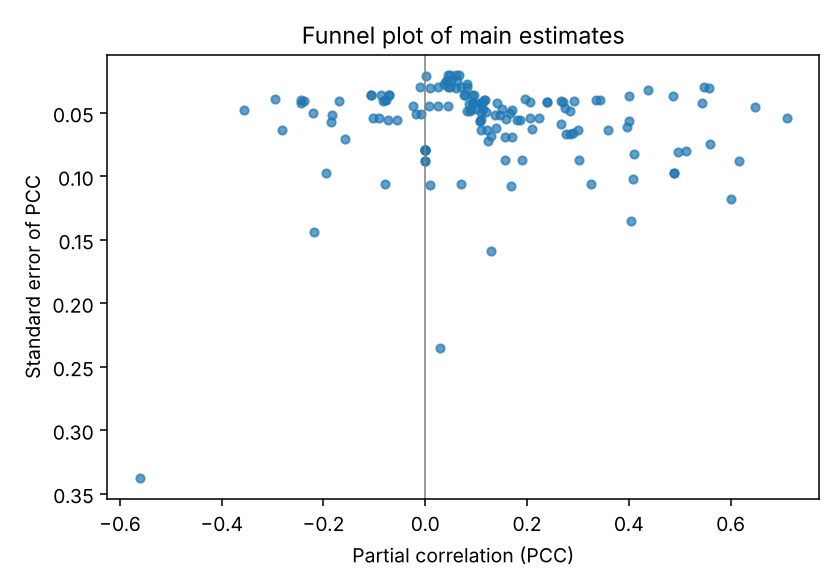
\includegraphics[width=0.58\textwidth]{../review/figures/funnel.png}
\caption{Funnel plot of main estimates (partial correlation against its standard error).}\label{fig:funnel}
\end{figure}

\section{Macro-panel data and additional results}\label{app:panel}
\subsection*{Variables}
\begin{table}[!ht]\centering\footnotesize\caption{World Bank WDI indicators used.}\label{tab:wdi}\begin{tabular}{@{}lll@{}}\toprule Role & Variable & WDI code\\\midrule
Technology & Mobile cellular subscriptions per 100 people & IT.CEL.SETS.P2\\
Technology & Individuals using the internet, \% of population & IT.NET.USER.ZS\\
Technology & Fixed broadband subscriptions per 100 people & IT.NET.BBND.P2\\
Outcome & GDP per capita, constant 2015 US\$ & NY.GDP.PCAP.KD\\
Outcome & Life expectancy at birth & SP.DYN.LE00.IN\\
Outcome & Under-5 mortality rate & SH.DYN.MORT\\
Outcome & Unemployment, \% of labour force & SL.UEM.TOTL.ZS\\
Outcome & Agriculture, value added \% of GDP & NV.AGR.TOTL.ZS\\
Outcome & Electric power consumption per capita & EG.USE.ELEC.KH.PC\\
Control or moderator & School enrolment, secondary, gross & SE.SEC.ENRR\\
Control & Trade, \% of GDP & NE.TRD.GNFS.ZS\\
Moderator & Domestic credit to private sector, \% of GDP & FS.AST.PRVT.GD.ZS\\
Moderator & Access to electricity, \% of population & EG.ELC.ACCS.ZS\\
Other & Population, total & SP.POP.TOTL\\
\bottomrule\end{tabular}\end{table}

Income groups follow the World Bank's current classification of 217 economies (25 low, 47 lower-middle, 59 upper-middle and 86 high income; the analysis sample is smaller because of missing data). Aggregates were removed. CO$_2$ emissions per capita could not be retrieved from the API and are not analysed.

\begin{table}[!ht]\centering\footnotesize
\caption{Dose-response (A3): change in annual growth (pp) per +10 mobile subscriptions per 100, by baseline adoption level.}\label{tab:a3}
\begin{adjustbox}{max width=\linewidth}\begin{tabular}{@{}lrrp{6.4cm}@{}}\toprule
Sample & Baseline bin & Obs & Effect of +10 on annual growth (pp) \\ \midrule
All economies & <10 & 186 & 0.405 [0.249, 0.561] (p=0.00) \\
All economies & 10-40 & 97 & 0.281 [0.167, 0.395] (p=0.00) \\
All economies & 40-80 & 123 & 0.179 [0.059, 0.298] (p=0.00) \\
All economies & >80 & 249 & 0.271 [0.119, 0.423] (p=0.00) \\
Low and lower-middle income & <10 & 109 & 0.509 [0.171, 0.846] (p=0.00) \\
Low and lower-middle income & 10-40 & 36 & 0.359 [0.106, 0.612] (p=0.01) \\
Low and lower-middle income & 40-80 & 53 & 0.453 [0.080, 0.826] (p=0.02) \\
Low and lower-middle income & >80 & 35 & 1.367 [-0.005, 2.739] (p=0.05) \\
Upper-middle and high income & <10 & 77 & 0.234 [0.013, 0.455] (p=0.04) \\
Upper-middle and high income & 10-40 & 61 & 0.233 [0.093, 0.372] (p=0.00) \\
Upper-middle and high income & 40-80 & 70 & 0.120 [-0.008, 0.247] (p=0.07) \\
Upper-middle and high income & >80 & 214 & 0.159 [0.052, 0.266] (p=0.00) \\
\bottomrule\end{tabular}\end{adjustbox}\end{table}

\begin{table}[!ht]\centering\footnotesize
\caption{Differences inside low and lower-middle income economies (A6).}\label{tab:a6}
\begin{adjustbox}{max width=\linewidth}\begin{tabular}{@{}lll@{}}\toprule
Moderator (at start of period) & Interaction with +10 mobile (pp growth per SD) & Obs \\ \midrule
secondary enrolment & 0.136 [-0.205, 0.478] (p=0.43) & 233 \\
electricity access & 0.024 [-0.301, 0.348] (p=0.89) & 224 \\
private credit & -0.074 [-0.295, 0.147] (p=0.51) & 204 \\
log GDP per capita & 0.237 [-0.128, 0.602] (p=0.20) & 233 \\
\bottomrule\end{tabular}\end{adjustbox}\end{table}

\begin{table}[!ht]\centering\footnotesize
\caption{Event study, secondary outcomes (takeoff at 10 per 100): effects at five and ten years. Rows marked fails do not pass the pre-trend rule and are not interpreted.}\label{tab:essec}
\begin{adjustbox}{max width=\linewidth}\begin{tabular}{@{}llllll@{}}\toprule
Outcome & Sample & Treated & Pre-trend mean [95\% CI] & Effect at +5 & Effect at +10 \\ \midrule
Life expectancy (years) & All economies & 178 & 0.05 [-0.00, 0.08] (passes) & 0.86 [0.10, 1.69] & 3.12 [0.87, 8.04] \\
Life expectancy (years) & Low and lower-middle income & 66 & 0.03 [-0.07, 0.11] (passes) & 2.61 [-0.49, 6.38] & n/a \\
Life expectancy (years) & Upper-middle income & 56 & 0.05 [-0.03, 0.13] (passes) & 0.63 [-0.30, 1.78] & -1.50 [-3.98, 8.11] \\
Life expectancy (years) & High income & 56 & 0.02 [-0.08, 0.18] (passes) & 0.81 [0.02, 1.54] & 3.54 [1.09, 7.64] \\
Under-5 mortality (log x 100) & All economies & 178 & -0.09 [-0.35, 0.28] (passes) & -4.71 [-13.90, 1.67] & -21.07 [-82.86, -1.01] \\
Under-5 mortality (log x 100) & Low and lower-middle income & 66 & -0.20 [-0.72, 0.54] (passes) & -15.08 [-26.03, 1.04] & n/a \\
Under-5 mortality (log x 100) & Upper-middle income & 56 & 0.02 [-0.57, 0.53] (passes) & -2.97 [-21.71, 6.62] & -16.04 [-64.54, 21.92] \\
Under-5 mortality (log x 100) & High income & 56 & 0.21 [-0.47, 0.65] (passes) & -4.01 [-12.47, 4.85] & -22.43 [-83.11, -1.44] \\
Unemployment (pp) & All economies & 178 & 0.11 [0.01, 0.21] (fails) & -0.22 [-1.24, 0.71] & -0.67 [-2.55, 1.30] \\
Unemployment (pp) & Low and lower-middle income & 66 & -0.16 [-0.30, -0.03] (fails) & n/a & n/a \\
Unemployment (pp) & Upper-middle income & 56 & 0.54 [0.23, 0.74] (fails) & 1.34 [-1.33, 2.94] & n/a \\
Unemployment (pp) & High income & 56 & 0.01 [-0.27, 0.37] (passes) & -1.14 [-2.34, -0.07] & -0.67 [-2.75, 1.43] \\
Agriculture share of value added (pp) & All economies & 178 & 0.27 [0.02, 0.62] (fails) & -3.56 [-6.14, -1.16] & -10.42 [-19.91, -1.93] \\
Agriculture share of value added (pp) & Low and lower-middle income & 66 & 0.34 [-0.22, 1.05] (passes) & n/a & n/a \\
Agriculture share of value added (pp) & Upper-middle income & 56 & 0.36 [-0.05, 0.74] (passes) & -4.29 [-8.59, -0.54] & n/a \\
Agriculture share of value added (pp) & High income & 56 & 0.16 [-0.19, 0.52] (passes) & -3.24 [-5.71, -1.03] & -10.42 [-20.97, -1.85] \\
Electric power use per capita (log x 100) & All economies & 178 & 0.01 [-1.09, 1.04] (passes) & 10.26 [-3.84, 25.08] & 4.64 [-44.79, 61.92] \\
Electric power use per capita (log x 100) & Low and lower-middle income & 66 & -0.44 [-2.49, 1.76] (passes) & n/a & n/a \\
Electric power use per capita (log x 100) & Upper-middle income & 56 & -0.46 [-1.98, 2.11] (passes) & 2.12 [-17.66, 21.16] & n/a \\
Electric power use per capita (log x 100) & High income & 56 & 0.43 [-0.98, 1.21] (passes) & 14.04 [-1.25, 28.06] & 4.64 [-50.29, 58.52] \\
\bottomrule\end{tabular}\end{adjustbox}\end{table}


\subsection*{Fixed-effects panels, dose-response and differences inside low-income economies}
\subsection{Mobile adoption and growth by income group (A1, A2)}
Table~\ref{tab:panel} shows that a 10-subscription increase in mobile adoption per 100 people goes with higher annual growth in all four income groups over the same five-year period. The association is largest in lower-middle income economies (0.47 percentage points, 95\% CI 0.16 to 0.77) and about 0.16 in upper-middle and high-income economies; the low-income estimate (0.36) is imprecise (CI $-0.05$ to 0.76, 20 economies). With country fixed effects, the lower-middle estimate remains (0.36, $p=0.03$), and the others move toward 0.13 to 0.20.

The predetermined specification, which uses the previous period's change, does not reproduce this pattern: the association is positive only in lower-middle income economies (0.26, $p=0.02$), near zero in upper-middle, and negative in low-income ($-0.38$, $p=0.13$) and high-income ($-0.16$, $p=0.01$) economies, and negative in every income group for internet use. The contemporaneous associations therefore partly reflect growth driving adoption or shared shocks, and they should not be read as a payoff to adoption.

\begin{table}[ht]\centering\small
\caption{Mobile adoption and annual GDP-per-capita growth by income group: change in annual growth (percentage points) per +10 subscriptions per 100 people, five-year periods 1995--2019 (95\% CI; standard errors clustered by country).}\label{tab:panel}
\begin{tabular}{@{}lrrr@{}}\toprule
Income group & Economies & Same period (A1) & Previous period (A2)\\\midrule
Low & 20 & 0.36 [$-0.05$, 0.76] & $-0.38$ [$-0.86$, 0.11]\\
Lower-middle & 42 & 0.47 [0.16, 0.77] & 0.26 [0.03, 0.49]\\
Upper-middle & 51 & 0.16 [0.04, 0.28] & 0.01 [$-0.15$, 0.16]\\
High & 64 & 0.16 [0.05, 0.26] & $-0.16$ [$-0.28$, $-0.03$]\\\bottomrule
\end{tabular}\end{table}

\subsection{Dose-response and differences inside low-income economies (A3, A6)}
Across baseline adoption levels, the association is largest where adoption was below 10 per 100 (0.41) and smaller at 40 to 80 (0.18); it is not monotone, since it is 0.27 above 80 per 100. For low and lower-middle income economies the point estimate above 80 per 100 is the largest (1.37) but imprecise (95\% CI $-0.01$ to 2.74, 35 observations; Appendix Table~\ref{tab:a3}). Inside low and lower-middle income economies, none of initial secondary enrolment, electricity access, private credit or initial income significantly changed the association (all $p>0.19$; Appendix Table~\ref{tab:a6}); the intervals are wide, and a standard-deviation change in a moderator could change the association by about 0.3 percentage points in either direction.

\subsection{Event study around mobile takeoff (A4b)}
The first event-study design, stacked cohorts with controls that adopt more than ten years later or never, was not interpretable (Section~\ref{sec:methods}, Appendix~\ref{app:amend}): nearly every economy crosses the threshold in the window, only 7 clean controls existed for the low and lower-middle income group, and that group showed a pre-trend of 12 log points. The replacement design compares each cohort with economies not yet treated at each horizon and adjusts for initial income and earlier growth. It passes the pre-trend rule in all four samples when the takeoff threshold is 10 subscriptions per 100 (mean placebo effect between $-0.9$ and $0.6$ log points, all intervals including zero; Table~\ref{tab:event}).

\begin{table}[ht]\centering\small
\caption{Event study around the year mobile subscriptions reach 10 per 100 people: effect on log GDP per capita ($\times100$) relative to the year before takeoff and to economies not yet treated (95\% bootstrap interval, 400 draws). Pre-trend: mean of the placebo effects at $-5$ to $-2$ years.}\label{tab:event}
\begin{tabular}{@{}lrlll@{}}\toprule
Sample & Treated & Pre-trend & Effect at +5 years & Effect at +10 years\\\midrule
All economies & 178 & $-0.0$ [$-0.6$, 0.4] & 13.5 [0.6, 36.5] & 47.8 [$-12.5$, 149.1]\\
Low and lower-middle & 66 & 0.6 [$-0.6$, 1.6] & $-5.9$ [$-18.6$, 31.9] & not estimable\\
Upper-middle & 56 & $-0.9$ [$-2.0$, 0.3] & 11.9 [$-8.0$, 46.7] & 12.2 [$-70.1$, 118.6]\\
High & 56 & $-0.4$ [$-1.2$, 0.5] & 19.1 [6.2, 36.7] & 53.8 [4.2, 152.6]\\\bottomrule
\end{tabular}\end{table}

\begin{figure}[ht]\centering
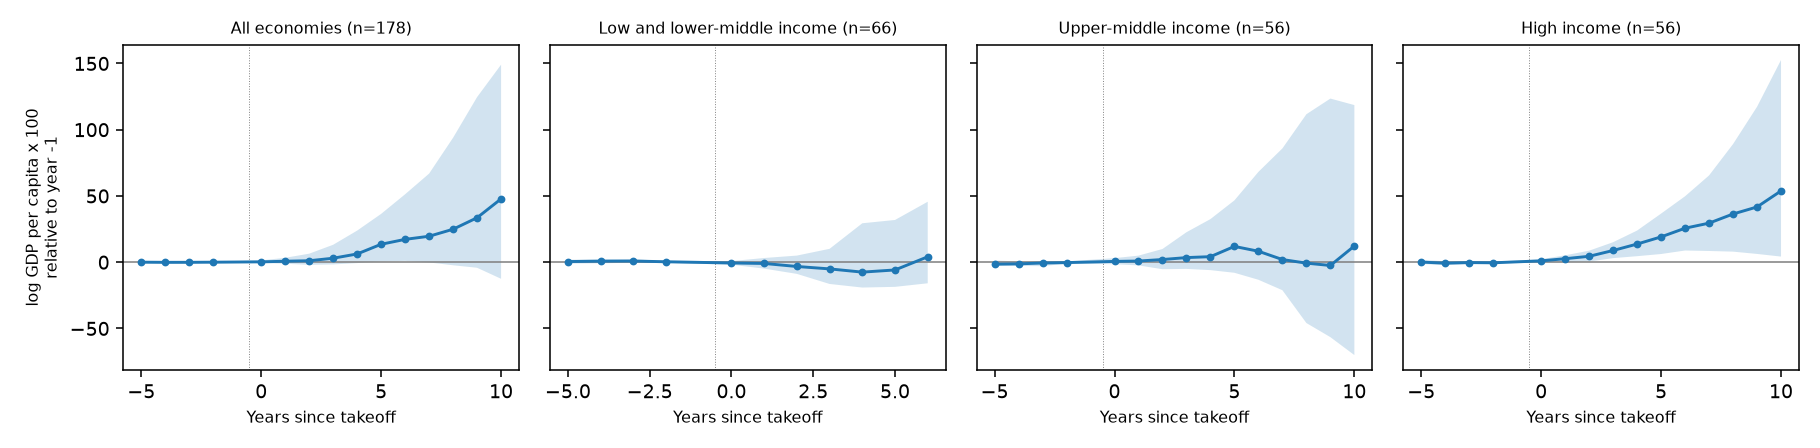
\includegraphics[width=\textwidth]{fig_event.png}
\caption{Event-study estimates by income group (takeoff at 10 mobile subscriptions per 100; shaded: 95\% bootstrap interval). The low and lower-middle panel stops at six years because fewer than eight not-yet-treated economies exist at longer horizons.}\label{fig:event}
\end{figure}

Economies that reach 10 subscriptions per 100 earlier have higher GDP per capita five years later than comparable economies that reach it later, by about 14 log points (95\% CI 0.6 to 36.5). The difference is distinguishable from zero only for high-income economies (19 log points, CI 6.2 to 36.7); the interval for low and lower-middle income economies, $-18.6$ to $+31.9$, is wide enough to contain effects of either sign and of the high-income size. Magnitudes at ten years (about 48 log points overall) are implausibly large for an effect of mobile telephony alone. They mainly show that economies reaching the threshold early are on different growth paths from those reaching it later, in ways initial income and earlier growth do not capture, and that at long horizons only the earliest cohorts contribute. The results are similar with a threshold of 25 per 100 (high income: 15.7 at five years, CI 6.5 to 28.8; low and lower-middle: $-7.5$, CI $-17.6$ to 13.3). With a threshold of 50, the pooled sample and the upper-middle sample fail the pre-trend rule and are not interpreted; the low and lower-middle estimate is 4.3 (CI $-10.7$ to 13.9) and the high-income estimate 8.9 (CI $-0.8$ to 20.8).

\emph{Outcomes beyond income.} For samples that pass the pre-trend rule, life expectancy is about 0.9 years higher five years after takeoff in the pooled sample (CI 0.1 to 1.7) and 0.8 years in high-income economies (CI 0.0 to 1.5), with a larger but imprecise estimate for low and lower-middle income economies (2.6 years, CI $-0.5$ to 6.4). Under-5 mortality is 15 log points lower in low and lower-middle income economies (CI $-26.0$ to 1.0). Unemployment and the agriculture share fail the pre-trend rule in most samples, and electricity use is not distinguishable from zero (Appendix Table~\ref{tab:essec}). These outcomes have strong secular trends, so we read these as descriptive.

\subsection{Local projections (A7)}
Local projections give a dynamic profile without a binary treatment (Table~\ref{tab:lp}, Figure~\ref{fig:lp}). For lower-middle income economies, a 10-subscription increase over three years is followed by cumulative growth that is higher by 0.41 percentage points after one year and by 2.0 points after six years (CI 0.8 to 3.2), then 1.7 after eight. For upper-middle and high-income economies, the profile is flat, and the high-income point estimate turns slightly negative (cumulative $-0.5$ after eight years, CI $-1.2$ to 0.2). For low-income economies the profile starts positive and turns negative ($-4.3$ after eight years, CI $-9.2$ to 0.6), but the intervals include zero except as noted. The placebo (future adoption against past growth) is close to zero in every group, though with a wide interval for low-income economies ($-0.75$, CI $-2.5$ to 1.0).

\begin{table}[ht]\centering\small
\caption{Local projections: cumulative growth of GDP per capita (percentage points) $h$ years after a +10 change in mobile subscriptions per 100 over the previous three years (95\% CI; country and year fixed effects).}\label{tab:lp}
\begin{tabular}{@{}lrllll@{}}\toprule
Group & Economies & $h=1$ & $h=2$ & $h=4$ & $h=8$\\\midrule
Low & 24 & 0.25 [$-0.08$, 0.58] & 0.34 [$-0.35$, 1.04] & $-0.44$ [$-2.23$, 1.35] & $-4.31$ [$-9.19$, 0.57]\\
Lower-middle & 47 & 0.41 [0.11, 0.71] & 0.76 [0.25, 1.27] & 1.51 [0.69, 2.33] & 1.69 [0.32, 3.07]\\
Upper-middle & 58 & $-0.00$ [$-0.21$, 0.21] & 0.10 [$-0.19$, 0.38] & 0.22 [$-0.45$, 0.88] & 0.17 [$-0.99$, 1.34]\\
High & 74 & 0.08 [$-0.04$, 0.19] & 0.06 [$-0.16$, 0.29] & $-0.06$ [$-0.48$, 0.35] & $-0.51$ [$-1.23$, 0.20]\\\bottomrule
\end{tabular}\end{table}

\begin{figure}[ht]\centering
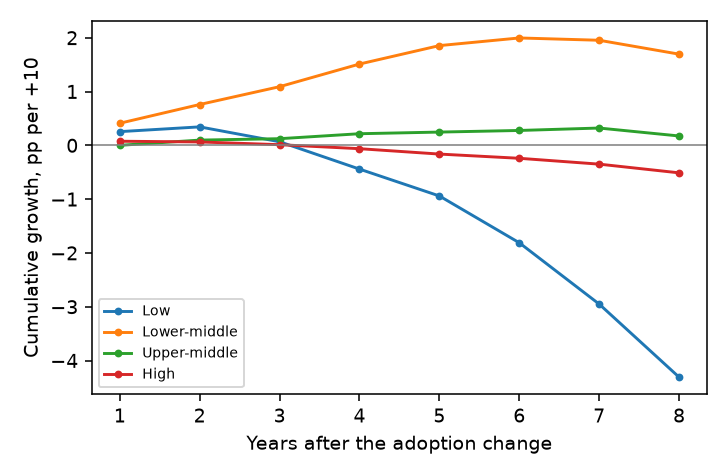
\includegraphics[width=0.6\textwidth]{fig_lp.png}
\caption{Local-projection profiles by income group.}\label{fig:lp}
\end{figure}

\subsection{Consistency across designs}
Table~\ref{tab:designs} summarises which income group shows a positive association under each design. No group is positive under all four. Lower-middle income economies are positive under three (A1, A2, local projections); under the event study they are pooled with low-income economies and the pooled estimate is null with a negative point estimate. High-income economies are positive under the same-period regression and the event study, but flat or negative under the predetermined regression and the local projections. Upper-middle economies are positive only in the same-period regression. Low-income economies are never significantly positive. We conclude that the panel analysis does not support a statement that richer or poorer economies gain more; the answer depends on the design, which is the same message as in the reviewed studies.

\begin{table}[ht]\centering\small
\caption{Direction and significance of the association between mobile adoption and GDP per capita growth, by design and income group (+ positive and significant at 5\%, $-$ negative and significant, 0 not significant; sign of the point estimate in parentheses).}\label{tab:designs}
\begin{tabular}{@{}lllll@{}}\toprule
Design & Low & Lower-middle & Upper-middle & High\\\midrule
A1 same period & 0 (+) & + & + & +\\
A2 previous period & 0 ($-$) & + & 0 (+) & $-$\\
Event study (+5 years) & \multicolumn{2}{c}{0 ($-$), low and lower-middle pooled} & 0 (+) & +\\
Local projections ($h=6$) & 0 ($-$) & + & 0 (+) & 0 ($-$)\\\bottomrule
\end{tabular}\end{table}



\section{Protocol amendments}\label{app:amend}
\small
\begin{enumerate}[leftmargin=1.6em,itemsep=2pt]
\item (2 Oct 2026) The OpenAlex query was written with explicit phrase variants and restricted to the economics field, because an unrestricted query returned about 7,600 records, too many for one screener.
\item (2 Oct) Four holding categories were added at the abstract stage: context, environmental outcome only, reviews for backward citation search, and supplementary micro evidence.
\item (2 Oct) arXiv was attempted but not completed. Scopus, Web of Science and EconLit were not searched.
\item (2 Oct) Automated stage-1 rules were added before manual reading, with a single assisted screener and a verification sample of 90 decisions.
\item (2 Oct) Included records were ranked in two tiers to decide which paywalled studies to request first.
\item (2 Oct) Records with no free full text and not on the short request list were kept as an abstract-level evidence map, excluded from pooled estimates and from risk-of-bias ratings.
\item (3 Oct) Studies whose only available venue the author judged unreliable were not read and not used.
\item (3 Oct) Four studies (298, 474, 878 and 1495) were moved from include to exclude after the cross-check. Five regression estimates were excluded from the meta-regression after the cross-check.
\item (4 Oct) A blind re-screening of a random sample flagged missed records; five were obtained and read (448, 474, 755, 891, 9001), four were included and 474 was moved to exclude.
\item (4 Oct) Because the re-screening and then a first-page check of one Google Scholar query showed that the search had missed studies, the supplementary Google Scholar queries were added (G1 to G15; the four run are listed in Appendix~\ref{app:search}). Only the first pages of G1, G2, G4 and G7 have been run. Twenty-nine of their 40 results were new; twenty full texts were obtained and read (9101 to 9106, 9201 to 9204, 9301 to 9305, 9401 to 9404 and 1580), seventeen were included and three (9202, five countries; 9301, a model without estimation; 9403, estimated on a simulated panel) excluded. Pilot meta-regression, exploratory analyses and all counts were rerun after their inclusion, and the earlier moderator results were superseded. Further amendment (4 Oct): a G2 result removed by the automated stage-1 rule (Yin and Choi 2023) was recovered, showing that the stage-1 term list was too narrow.
\item (3 Oct) The event-study design in the macro-panel plan was replaced by a staggered design with not-yet-treated controls and covariate adjustment after the first design failed its pre-trend checks; local projections were added.
\end{enumerate}

\section{Reporting checklist (PRISMA 2020 items, used as a guide)}\label{app:prisma}
{\scriptsize\begin{longtable}{@{}l p{3.6cm} p{4.2cm} l p{4.6cm}@{}}
\caption{PRISMA 2020 checklist: where each item is reported. Section numbers refer to this paper.}\label{tab:prismacheck}\\
\toprule Item & Topic & Requirement & Reported & Where \\ \midrule \endfirsthead
\toprule Item & Topic & Requirement & Reported & Where \\ \midrule \endhead
\bottomrule \endfoot
1 & Title & Identifies the report type & Yes & Title \\
2 & Abstract & Structured abstract & Yes & Abstract \\
3--4 & Rationale, objectives & Context and explicit question & Yes & Sections 1--2 \\
5 & Eligibility criteria & Inclusion and exclusion & Yes & Section 3.2; Appendix D \\
6--7 & Sources, search strategy & Databases, dates, full strategy & Partly & Section 3.3; Appendix C \\
8 & Selection process & Screening method, reviewers & Partly & Section 3.4; one reviewer \\
9--10 & Data collection, items & Coding method and items & Yes & Section 3.5; Appendix D \\
11, 18 & Risk of bias & Tool, reviewers, results & Partly & Sections 3.7, 4.3; Appendix A \\
12--14 & Effect measures, synthesis & Measures and methods & Yes & Section 3.6; Appendices E, F \\
15, 22 & Certainty of evidence & GRADE or similar & No & Not done; see Limitations \\
16--21 & Results & Flow, studies, bias, synthesis & Yes & Section 4; Appendices A, B \\
23--27 & Discussion, declarations & Limits, protocol, funding, data & Partly & Sections 5--6; Declarations \\
\end{longtable}}

\end{document}
